\documentclass[8pt,fleqn,openany]{book}
\usepackage[utf8]{inputenc}
\usepackage[top=3cm,bottom=3cm,left=3.2cm,right=3.2cm,headsep=16pt,letterpaper]{geometry}
\usepackage{xcolor}
\definecolor{defaultcolor}{RGB}{38,131,255}
\definecolor{ForestGreen}{RGB}{34,139,34}
\usepackage{tabulary}

\usepackage{hyperref} \def\UrlBreaks{\do\/\do-}
\usepackage{graphicx}
\usepackage[english]{babel}
\usepackage{listings}
\usepackage{listings-golang}
\usepackage{listings-protobuf}
\usepackage{color}
\usepackage{tikz}
\usepackage[labelfont=it,textfont={it},singlelinecheck=on,justification=centering]{caption}
\usepackage{amsmath}
\usepackage{float}
\usepackage{comment}
\usepackage{cite}
\usepackage{placeins}
\usepackage{tabulary}

\usepackage{inconsolata}
\usepackage[defaultfam,light]{montserrat}
\usepackage[italic]{mathastext}

\setlength{\parskip}{1em}
\urlstyle{rm}
\renewcommand{\rmdefault}{Montserrat-LF}

\renewcommand{\baselinestretch}{1.15}

\newcommand{\code}[1]{{\em #1}}

\lstset{
    basicstyle=\footnotesize\tt,
    keywordstyle=\color{blue},
    numbers=left,
    numbersep=5pt,
    showstringspaces=false,
    stringstyle=\color{red},
    commentstyle=\color{ForestGreen},
    tabsize=2,
    language=Golang
}

\title{\textbf{\sffamily\color{white} \
Storj: A Decentralized Cloud Storage Network Framework}}
\author{\small\sffamily\color{white}
Storj Labs, Inc.}
\date{\small\sffamily\color{white} v3.0, October 13, 2018\\
\small\colorlet{urllinkcolor}{white}\url{https://github.com/storj/whitepaper}
}

%----------------------------------------------------------------------------------------
%	VARIOUS REQUIRED PACKAGES
%----------------------------------------------------------------------------------------

\usepackage{titlesec} % Allows customization of titles

\graphicspath{{Pictures/}} % Specifies the directory where pictures are stored

\usepackage{enumitem} % Customize lists
\setlist{nolistsep} % Reduce spacing between bullet points and numbered lists

\usepackage{booktabs} % Required for nicer horizontal rules in tables

\usepackage{eso-pic} % Required for specifying an image background in the title page

%----------------------------------------------------------------------------------------
%	MAIN TABLE OF CONTENTS
%----------------------------------------------------------------------------------------

\usepackage{titletoc} % Required for manipulating the table of contents

\contentsmargin{0cm} % Removes the default margin
% Chapter text styling
\titlecontents{chapter}[1.25cm] % Indentation
{\addvspace{15pt}\large\sffamily\bfseries} % Spacing and font options for chapters
{\color{ocre!60}\contentslabel[\Large\thecontentslabel]{1.25cm}\color{ocre}} % Chapter number
{}
{\color{ocre!60}\normalsize\sffamily\bfseries\;\titlerule*[.5pc]{.}\;\thecontentspage} % Page number
% Section text styling
\titlecontents{section}[1.25cm] % Indentation
{\addvspace{5pt}\sffamily\bfseries} % Spacing and font options for sections
{\contentslabel[\thecontentslabel]{1.25cm}} % Section number
{}
{\sffamily\hfill\color{black}\thecontentspage} % Page number
[]
% Subsection text styling
\titlecontents{subsection}[1.25cm] % Indentation
{\addvspace{1pt}\sffamily\small} % Spacing and font options for subsections
{\contentslabel[\thecontentslabel]{1.25cm}} % Subsection number
{}
{\sffamily\;\titlerule*[.5pc]{.}\;\thecontentspage} % Page number
[]

%----------------------------------------------------------------------------------------
%	MINI TABLE OF CONTENTS IN CHAPTER HEADS
%----------------------------------------------------------------------------------------

% Section text styling
\titlecontents{lsection}[0em] % Indendating
{\footnotesize\sffamily} % Font settings
{}
{}
{}

% Subsection text styling
\titlecontents{lsubsection}[.5em] % Indentation
{\normalfont\footnotesize\sffamily} % Font settings
{}
{}
{}

%----------------------------------------------------------------------------------------
%	PAGE HEADERS
%----------------------------------------------------------------------------------------

\usepackage{fancyhdr} % Required for header and footer configuration

\pagestyle{fancy}
\renewcommand{\chaptermark}[1]{\markboth{\sffamily\normalsize\bfseries\chaptername\ \thechapter.\ #1}{}} % Chapter text font settings
\renewcommand{\sectionmark}[1]{\markright{\sffamily\normalsize\thesection\hspace{5pt}#1}{}} % Section text font settings
\fancyhf{} \fancyhead[LE,RO]{\sffamily\normalsize\thepage} % Font setting for the page number in the header
\fancyhead[LO]{\rightmark} % Print the nearest section name on the left side of odd pages
\fancyhead[RE]{\leftmark} % Print the current chapter name on the right side of even pages
\renewcommand{\headrulewidth}{0.5pt} % Width of the rule under the header
\addtolength{\headheight}{2.5pt} % Increase the spacing around the header slightly
\renewcommand{\footrulewidth}{0pt} % Removes the rule in the footer
\fancypagestyle{plain}{\fancyhead{}\renewcommand{\headrulewidth}{0pt}} % Style for when a plain pagestyle is specified

% Removes the header from odd empty pages at the end of chapters
\makeatletter
\renewcommand{\cleardoublepage}{
\clearpage\ifodd\c@page\else
\hbox{}
\vspace*{\fill}
\thispagestyle{empty}
\newpage
\fi}

%----------------------------------------------------------------------------------------
%	THEOREM STYLES
%----------------------------------------------------------------------------------------

\usepackage{amsmath,amsfonts,amssymb,amsthm} % For math equations, theorems, symbols, etc

\newcommand{\intoo}[2]{\mathopen{]}#1\,;#2\mathclose{[}}
\newcommand{\ud}{\mathop{\mathrm{{}d}}\mathopen{}}
\newcommand{\intff}[2]{\mathopen{[}#1\,;#2\mathclose{]}}
\newtheorem{notation}{Notation}[chapter]

%%%%%%%%%%%%%%%%%%%%%%%%%%%%%%%%%%%%%%%%%%%%%%%%%%%%%%%%%%%%%%%%%%%%%%%%%%%
%%%%%%%%%%%%%%%%%%%% dedicated to boxed/framed environements %%%%%%%%%%%%%%
%%%%%%%%%%%%%%%%%%%%%%%%%%%%%%%%%%%%%%%%%%%%%%%%%%%%%%%%%%%%%%%%%%%%%%%%%%%
\newtheoremstyle{ocrenumbox}% % Theorem style name
{0pt}% Space above
{0pt}% Space below
{\normalfont}% % Body font
{}% Indent amount
{\small\bf\sffamily\color{ocre}}% % Theorem head font
{\;}% Punctuation after theorem head
{0.25em}% Space after theorem head
{\small\sffamily\color{ocre}\thmname{#1}\nobreakspace\thmnumber{\@ifnotempty{#1}{}\@upn{#2}}% Theorem text (e.g. Theorem 2.1)
\thmnote{\nobreakspace\the\thm@notefont\sffamily\bfseries\color{black}---\nobreakspace#3.}} % Optional theorem note
\renewcommand{\qedsymbol}{$\blacksquare$}% Optional qed square

\newtheoremstyle{blacknumex}% Theorem style name
{5pt}% Space above
{5pt}% Space below
{\normalfont}% Body font
{} % Indent amount
{\small\bf\sffamily}% Theorem head font
{\;}% Punctuation after theorem head
{0.25em}% Space after theorem head
{\small\sffamily{\tiny\ensuremath{\blacksquare}}\nobreakspace\thmname{#1}\nobreakspace\thmnumber{\@ifnotempty{#1}{}\@upn{#2}}% Theorem text (e.g. Theorem 2.1)
\thmnote{\nobreakspace\the\thm@notefont\sffamily\bfseries---\nobreakspace#3.}}% Optional theorem note

\newtheoremstyle{blacknumbox} % Theorem style name
{0pt}% Space above
{0pt}% Space below
{\normalfont}% Body font
{}% Indent amount
{\small\bf\sffamily}% Theorem head font
{\;}% Punctuation after theorem head
{0.25em}% Space after theorem head
{\small\sffamily\thmname{#1}\nobreakspace\thmnumber{\@ifnotempty{#1}{}\@upn{#2}}% Theorem text (e.g. Theorem 2.1)
\thmnote{\nobreakspace\the\thm@notefont\sffamily\bfseries---\nobreakspace#3.}}% Optional theorem note

%%%%%%%%%%%%%%%%%%%%%%%%%%%%%%%%%%%%%%%%%%%%%%%%%%%%%%%%%%%%%%%%%%%%%%%%%%%
%%%%%%%%%%%%% dedicated to non-boxed/non-framed environements %%%%%%%%%%%%%
%%%%%%%%%%%%%%%%%%%%%%%%%%%%%%%%%%%%%%%%%%%%%%%%%%%%%%%%%%%%%%%%%%%%%%%%%%%
\newtheoremstyle{ocrenum}% % Theorem style name
{5pt}% Space above
{5pt}% Space below
{\normalfont}% % Body font
{}% Indent amount
{\small\bf\sffamily\color{ocre}}% % Theorem head font
{\;}% Punctuation after theorem head
{0.25em}% Space after theorem head
{\small\sffamily\color{ocre}\thmname{#1}\nobreakspace\thmnumber{\@ifnotempty{#1}{}\@upn{#2}}% Theorem text (e.g. Theorem 2.1)
\thmnote{\nobreakspace\the\thm@notefont\sffamily\bfseries\color{black}---\nobreakspace#3.}} % Optional theorem note
\renewcommand{\qedsymbol}{$\blacksquare$}% Optional qed square
\makeatother

% Defines the theorem text style for each type of theorem to one of the three styles above
\newcounter{dummy}
\numberwithin{dummy}{section}
\theoremstyle{ocrenumbox}
\newtheorem{theoremeT}[dummy]{Theorem}
\newtheorem{problem}{Problem}[chapter]
\newtheorem{exerciseT}{Exercise}[chapter]
\theoremstyle{blacknumex}
\newtheorem{exampleT}{Example}[chapter]
\theoremstyle{blacknumbox}
\newtheorem{vocabulary}{Vocabulary}[chapter]
\newtheorem{definitionT}{Definition}[section]
\newtheorem{corollaryT}[dummy]{Corollary}
\theoremstyle{ocrenum}
\newtheorem{proposition}[dummy]{Proposition}

%----------------------------------------------------------------------------------------
%	DEFINITION OF COLORED BOXES
%----------------------------------------------------------------------------------------

\RequirePackage[framemethod=default]{mdframed} % Required for creating the theorem, definition, exercise and corollary boxes

% Theorem box
\newmdenv[skipabove=7pt,
skipbelow=7pt,
backgroundcolor=black!5,
linecolor=ocre,
innerleftmargin=5pt,
innerrightmargin=5pt,
innertopmargin=5pt,
leftmargin=0cm,
rightmargin=0cm,
innerbottommargin=5pt]{tBox}

% Exercise box
\newmdenv[skipabove=7pt,
skipbelow=7pt,
rightline=false,
leftline=true,
topline=false,
bottomline=false,
backgroundcolor=ocre!10,
linecolor=ocre,
innerleftmargin=5pt,
innerrightmargin=5pt,
innertopmargin=5pt,
innerbottommargin=5pt,
leftmargin=0cm,
rightmargin=0cm,
linewidth=4pt]{eBox}

% Definition box
\newmdenv[skipabove=7pt,
skipbelow=7pt,
rightline=false,
leftline=true,
topline=false,
bottomline=false,
linecolor=ocre,
innerleftmargin=5pt,
innerrightmargin=5pt,
innertopmargin=0pt,
leftmargin=0cm,
rightmargin=0cm,
linewidth=4pt,
innerbottommargin=0pt]{dBox}

% Corollary box
\newmdenv[skipabove=7pt,
skipbelow=7pt,
rightline=false,
leftline=true,
topline=false,
bottomline=false,
linecolor=gray,
backgroundcolor=black!5,
innerleftmargin=5pt,
innerrightmargin=5pt,
innertopmargin=5pt,
leftmargin=0cm,
rightmargin=0cm,
linewidth=4pt,
innerbottommargin=5pt]{cBox}

% Creates an environment for each type of theorem and assigns it a theorem text style from the "Theorem Styles" section above and a colored box from above
\newenvironment{theorem}{\begin{tBox}\begin{theoremeT}}{\end{theoremeT}\end{tBox}}
\newenvironment{exercise}{\begin{eBox}\begin{exerciseT}}{\hfill{\color{ocre}\tiny\ensuremath{\blacksquare}}\end{exerciseT}\end{eBox}}
\newenvironment{definition}{\begin{dBox}\begin{definitionT}}{\end{definitionT}\end{dBox}}
\newenvironment{example}{\begin{exampleT}}{\hfill{\tiny\ensuremath{\blacksquare}}\end{exampleT}}
\newenvironment{corollary}{\begin{cBox}\begin{corollaryT}}{\end{corollaryT}\end{cBox}}

%----------------------------------------------------------------------------------------
%	REMARK ENVIRONMENT
%----------------------------------------------------------------------------------------

\newenvironment{remark}{\par\vspace{10pt}\small % Vertical white space above the remark and smaller font size
\begin{list}{}{
\leftmargin=35pt % Indentation on the left
\rightmargin=25pt}\item\ignorespaces % Indentation on the right
\makebox[-2.5pt]{\begin{tikzpicture}[overlay]
\node[draw=ocre!60,line width=1pt,circle,fill=ocre!25,font=\sffamily\bfseries,inner sep=2pt,outer sep=0pt] at (-15pt,0pt){\textcolor{ocre}{R}};\end{tikzpicture}} % Orange R in a circle
\advance\baselineskip -1pt}{\end{list}\vskip5pt} % Tighter line spacing and white space after remark

%----------------------------------------------------------------------------------------
%	SECTION NUMBERING IN THE MARGIN
%----------------------------------------------------------------------------------------

\makeatletter
\renewcommand{\@seccntformat}[1]{\llap{\textcolor{ocre}{\csname the#1\endcsname}\hspace{1em}}}
\renewcommand{\section}{\@startsection{section}{1}{\z@}
{-4ex \@plus -1ex \@minus -.4ex}
{1ex \@plus.2ex }
{\normalfont\large\sffamily\bfseries}}
\renewcommand{\subsection}{\@startsection {subsection}{2}{\z@}
{-3ex \@plus -0.1ex \@minus -.4ex}
{0.5ex \@plus.2ex }
{\normalfont\sffamily\bfseries}}
\renewcommand{\subsubsection}{\@startsection {subsubsection}{3}{\z@}
{-2ex \@plus -0.1ex \@minus -.2ex}
{.2ex \@plus.2ex }
{\normalfont\small\sffamily\bfseries}}
\renewcommand\paragraph{\@startsection{paragraph}{4}{\z@}
{-2ex \@plus-.2ex \@minus .2ex}
{.1ex}
{\normalfont\small\sffamily\bfseries}}

%----------------------------------------------------------------------------------------
%	HYPERLINKS IN THE DOCUMENTS
%----------------------------------------------------------------------------------------

% For an unclear reason, the package should be loaded now and not later
\usepackage{hyperref}
\hypersetup{hidelinks,backref=true,pagebackref=true,hyperindex=true,colorlinks=false,breaklinks=true,urlcolor= ocre,bookmarks=true,bookmarksopen=false,pdftitle={Title},pdfauthor={Author}}

%----------------------------------------------------------------------------------------
%	CHAPTER HEADINGS
%----------------------------------------------------------------------------------------

% The set-up below should be (sadly) manually adapted to the overall margin page septup controlled by the geometry package loaded in the main.tex document. It is possible to implement below the dimensions used in the goemetry package (top,bottom,left,right)... TO BE DONE

\newcommand{\thechapterimage}{}
\newcommand{\chapterimage}[1]{\renewcommand{\thechapterimage}{#1}}

% Numbered chapters with mini tableofcontents
\def\thechapter{\arabic{chapter}}
\def\@makechapterhead#1{
\thispagestyle{empty}
{\centering \normalfont\sffamily
\ifnum \c@secnumdepth >\m@ne
\if@mainmatter
\startcontents
\begin{tikzpicture}[remember picture,overlay]
\node at (current page.north west)
{\begin{tikzpicture}[remember picture,overlay]
\node[anchor=north west,inner sep=0pt] at (0,0) {\includegraphics[width=\paperwidth]{\thechapterimage}};
%%%%%%%%%%%%%%%%%%%%%%%%%%%%%%%%%%%%%%%%%%%%%%%%%%%%%%%%%%%%%%%%%%%%%%%%%%%%%%%%%%%%%
% Commenting the 3 lines below removes the small contents box in the chapter heading
%\fill[color=ocre!10!white,opacity=.6] (1cm,0) rectangle (8cm,-7cm);
%\node[anchor=north west] at (1.1cm,.35cm) {\parbox[t][8cm][t]{6.5cm}{\huge\bfseries\flushleft \printcontents{l}{1}{\setcounter{tocdepth}{2}}}};
\draw[anchor=west] (5cm,-9cm) node [rounded corners=20pt,fill=ocre!10!white,text opacity=1,draw=ocre,draw opacity=1,line width=1.5pt,fill opacity=.6,inner sep=12pt]{\huge\sffamily\bfseries\textcolor{black}{\thechapter. #1\strut\makebox[22cm]{}}};
%%%%%%%%%%%%%%%%%%%%%%%%%%%%%%%%%%%%%%%%%%%%%%%%%%%%%%%%%%%%%%%%%%%%%%%%%%%%%%%%%%%%%
\end{tikzpicture}};
\end{tikzpicture}}
\par\vspace*{230\p@}
\fi
\fi}

% Unnumbered chapters without mini tableofcontents (could be added though)
\def\@makeschapterhead#1{
\thispagestyle{empty}
{\centering \normalfont\sffamily
\ifnum \c@secnumdepth >\m@ne
\if@mainmatter
\begin{tikzpicture}[remember picture,overlay]
\node at (current page.north west)
{\begin{tikzpicture}[remember picture,overlay]
\node[anchor=north west,inner sep=0pt] at (0,0) {\includegraphics[width=\paperwidth]{\thechapterimage}};
\draw[anchor=west] (5cm,-9cm) node [rounded corners=20pt,fill=ocre!10!white,fill opacity=.6,inner sep=12pt,text opacity=1,draw=ocre,draw opacity=1,line width=1.5pt]{\huge\sffamily\bfseries\textcolor{black}{#1\strut\makebox[22cm]{}}};
\end{tikzpicture}};
\end{tikzpicture}}
\par\vspace*{230\p@}
\fi
\fi
}
\makeatother


\begin{document}

\raggedbottom
\widowpenalty10000
\clubpenalty10000

\thispagestyle{fancy}
\chapterimage{images/header.eps}
\AddToShipoutPicture*{\put(0,0){
\includegraphics[width=\paperwidth]{images/front.eps}}}

\maketitle

\begin{tikzpicture}[remember picture,overlay]
\node[rotate=45,scale=15,text opacity=0.1]
at (current page.center) {DRAFT};
\end{tikzpicture}

\newpage

\tableofcontents\newpage

\section{Abstract}

Decentralized cloud storage represents a fundamental shift in
the efficiency and economics of large-scale storage.
Eliminating central control allows users to store and share data
without reliance on a third-party storage provider. Decentralization mitigates
the risk of data failures and outages while simultaneously increasing
the security and privacy of object storage. It also
allows market forces to optimize for less expensive storage
at a greater rate than any single provider could afford.
Although there are many ways to build such a system, there are some specific
responsibilities any given implementation should address.
Based on our experience with petabyte-scale
storage systems, we introduce a modular framework for considering these
responsibilities and for building our distributed storage network.
Additionally, we describe an initial
concrete implementation for the entire framework.

\section{Contributors}

This paper represents the combined efforts of many individuals.
Contributors affiliated with Storj Labs, Inc. include but are not limited to:
Tim Adams,
Kishore Aligeti,
Cameron Ayer,
Atikh Bana,
Alexander Bender,
Stefan Benten,
Maximillian von Briesen,
Paul Cannon,
Gina Cooley,
Dennis Coyle,
Egon Elbre,
Nadine Farah,
Patrick Gerbes,
John Gleeson,
Ben Golub,
James Hagans,
Jens Heimbürge,
Faris Huskovic,
Philip Hutchins,
Brandon Iglesias,
Viktor Ihnatiuk,
Jennifer Johnson,
Kevin Leffew,
Alexander Leitner,
Richard Littauer,
Dylan Lott,
JT Olio,
Kaloyan Raev,
Garrett Ransom,
Matthew Robinson,
Jon Sanderson,
Benjamin Sirb,
Dan Sorensen,
Helene Unland,
Natalie Villasana,
Bryan White,
and Shawn Wilkinson.

We'd also like to especially thank the other authors and contributors of the
previous Storj v2 whitepaper:
Tome Boshevski,
Josh Brandoff,
Vitalik Buterin,
Braydon Fuller,
Gordon Hall,
Chris Pollard,
and James Prestwich.

We would like to acknowledge the efforts, whitepapers, and communications of
others in the distributed computing, blockchain, distributed storage, and
decentralized storage space, whose work has informed our efforts. A more
comprehensive list of sources is in the bibliography, but we would like to
provide particular acknowledgement to the teams that built
Allmydata,
Ceph,
CoralCDN,
Ethereum,
Filecoin,
Freenet,
Gluster,
GFS,
Hadoop,
IPFS,
Kademlia,
Lustre,
Maidsafe,
Minio,
MojoNation,
OceanStore,
Scality,
Siacoin,
and Tahoe-LAFS.

Finally, we extend a huge thank you to everyone we talked to during the
design and architecture of this system for their valuable thoughts, feedback,
input, and suggestions.

Please address correspondence to \href{mailto:paper@storj.io}{paper@storj.io}.

\chapter{Introduction}\label{chap:intro}

The Internet is a massive decentralized and distributed network consisting of
billions of devices which are not controlled by a single group or entity.
Much of the data currently available through the Internet is quite centralized
and is stored with a handful of technology companies that have the
experience and capital to build massive data centers capable of handling this
vast amount of information.
A few of the challenges faced by data centers are: data breaches, periods of
unavailability on a grand scale, storage costs, and expanding and upgrading quickly enough to meet user demand for faster data and larger formats.

Decentralized storage has emerged as an answer to the challenge of
providing a performant, secure, private, and economical cloud storage solution.
Decentralized storage is better positioned to achieve these outcomes as the
architecture has a more natural alignment to the decentralized architecture of
the Internet as a whole, as opposed to massive centralized data centers.

News coverage of data breaches over the past few years has shown us that the
frequency of data breaches has been increasing by as much as a factor of 10
between 2005 and 2017 \cite{breaches}.
Decentralized storage's process of protecting data makes data breaches more
difficult than current methods used by data centers while, at the same time,
costs less than current storage methods.

This model can address the rapidly
expanding amount of data for which current solutions struggle.
With an anticipated 44 zettabytes of data expected to exist by 2020 and a
market that will grow to \$92 billion USD in the same time frame
\cite{storage-growth}, we have identified several key market segments that decentralized cloud storage
has the potential to address.
As decentralized cloud storage capabilities evolve, it will be able to address a much wider range of use cases from basic
object storage to content delivery networks (CDN).

Decentralized cloud storage is rapidly advancing in maturity, but its evolution
is subject to a specific set of design constraints which
define the overall requirements and implementation of
the network. When designing a distributed storage system,
there are many parameters to be optimized such as speed, capacity,
trustlessness, byzantine fault tolerance, cost, bandwidth, and latency.

We propose a framework that scales horizontally to exabytes of data storage
across the globe. Our system, the Storj Network, is a robust object store
that encrypts, shards, and distributes data to nodes around the world for
storage.
Data is stored and served in a manner purposefully designed to prevent
breaches.
In order to accomplish this task, we've designed our system to be modular,
consisting of independent components with task-specific jobs.
We've integrated these components to implement a decentralized object storage
system that is not only secure, performant, and reliable but also significantly
more economical than either on premises or traditional, centralized cloud storage.

As with Google's Chubby lock service \cite{chubby}, the Storj Network is an
engineering effort required to fill the needs mentioned throughout this paper.
The concrete implementation detailed here was not research.
We claim no novel algorithms or techniques. The purpose
of this paper is to describe what we did, what we plan to do, and why we chose build it in this way.

We have organized the rest of this paper into six additional
chapters. Chapter \ref{chap:design-constraints} discusses the design space
in which Storj operates and the specific constraints on which
our optimization efforts are based.
Chapter \ref{chap:framework} covers our framework. Chapter
\ref{chap:concrete}
proposes a simple concrete implementation of each component,
while chapter \ref{chap:walkthroughs} explains what happens
during each operation in the network. Chapter
\ref{chap:future-work} covers future work.
Finally, chapter \ref{chap:selected-calcs} covers selected calculations.

\chapter{Storj design constraints}\label{chap:design-constraints}

Before designing a system, it's important to first define its requirements.
There are many different ways to design a decentralized storage system. However,
with the addition of a few requirements, the potential design space shrinks
significantly.
Our design constraints are heavily influenced by our product and
market fit goals.
By carefully considering each requirement, we ensure the framework
we choose is as universal as possible, given the constraints.

\section{Security and privacy}

Any object storage platform must ensure both the privacy and
security of data stored regardless of whether it is centralized or decentralized.
Decentralized storage platforms must mitigate an additional layer of
complexity and risk associated with the storage of data on inherently
untrusted nodes. Because decentralized storage platforms cannot take many
of the same shortcuts data center based approaches can (e.g. firewalls, DMZs,
etc.), decentralized storage must be designed from the ground up to support
not only end-to-end encryption but also enhanced security and privacy at all levels of the
system.

Certain categories of data are also subject to specific regulatory compliance.
For example, the United States legislation for
the Health Insurance Portability and
Accountability Act (HIPAA) has specific requirements for data center
compatibility. European countries have to consider the General Data Protection
Regulation (GDPR) regarding
how individual information must be protected and secured. There
are many other regulations in other sectors regarding user's data privacy.

Customers should be able to
evaluate that our software is implemented correctly, is resistant to
attack vectors (known or unknown), is secure, and otherwise fulfills all
of the customers' requirements.
Open source software
provides the level of transparency and assurance needed to prove that the
behaviors of the system are as advertised.

\section{Decentralization}

Informally, a decentralized application is a service that has no single
operator. Furthermore, no single entity should be solely responsible for the
cost associated with running the service.

One of the main motivations for preferring decentralization is to drive
down infrastructure costs for maintenance, utilities, and bandwidth.
We believe that there
are significant underutilized resources at the edge of the network
for many smaller operators. In our experience building decentralized
storage networks, we have found a long tail of resources that are presently
unused or underused that could provide affordable and
geographically distributed cloud storage. Conceivably, some small operator
has access to less expensive electricity than standard data centers or another small
operator has access to less expensive cooling. Many of these small operator
environments are not substantial enough to run an entire datacenter-like
storage system. For example, perhaps a rural hydro-electric dam operator has
enough excess electricity to run ten servers, but no more. We have found that
in aggregate, enough small operator environments exist such that their
combination over the internet constitutes
significant opportunity and advantage for less expensive and faster storage.

Our decentralization goals for fundamental infrastructure, such as storage, are also driven by our desire to provide a viable alternative to the few major
centralized storage entities who dominate the market at present.
We believe that there exists inherent risk in trusting a single entity,
company, or organization with a significant percentage of the world's data.
In fact, we believe that there is an implicit cost associated with the risk of
trusting any third party with custodianship of personal data.
Some possible costly outcomes include changes to the company's roadmap that could result in the product
becoming less useful, changes to the company's position on data collection that could
cause it to sell customer metadata to advertisers, or even the company could go
out of business or otherwise fail to keep customer data safe.
By creating an equivalent or better decentralized
system, many users concerned about single-entity risk will have a viable
alternative.
With decentralized architecture, Storj could cease operating and the data
would continue to be available.

We have decided to adopt a decentralized architecture because, despite the trade-offs, we believe decentralization better addresses the needs of cloud storage
and resolves many core limitations, risks, and cost factors that result from
centralization. Within this context,
decentralization results in a globally distributed network that can
serve a wide range of storage use cases from archival to CDN. Whereas,
centralized storage systems require different architectures, implementations,
and infrastructure to address each of those same use cases.

\section{Marketplace and economics}

Public cloud computing, and public cloud storage in particular, has
proven to be an attractive business model for the large centralized cloud
providers. Cloud computing is estimated to be a \$186.4 billion dollar market
in 2018, and reach \$302.5 billion by 2021 \cite{gartner-cloud-growth}.

The public cloud storage model has provided a compelling economic model to end
users. Not only does it enable end users to scale on demand but also it allows them to avoid the significant fixed costs of facilities, power, and data center
personnel. Public cloud storage has generally proven to be an economical,
durable, and performant option for many end users when compared to
on-premise solutions.

However, the public cloud storage model has, by its nature, led to a high
degree of concentration. Fixed costs are born by the network operators, who
invest billions of dollars in building out a network of data centers and
then enjoy significant economies of scale. The combination of large upfront
costs and economies of scale means that there is an extremely limited number
of viable suppliers of public cloud storage (arguably, fewer than five major
operators worldwide). These few suppliers are also the primary beneficiaries of
the economic return.

We believe that decentralized storage can provide a viable alternative to
centralized cloud.
However, to compel partners or customers to bring data to the network,
the price charged for storage and bandwidth---combined with the other
benefits of decentralized storage---must be
more compelling and economically beneficial than competing storage solutions.
In our design of Storj, we seek to create an economically advantageous
situation for four different groups:

\begin{description}
\item[End users] - We must provide the same economically compelling
  characteristics of public cloud storage with no upfront costs and scale on
  demand.
  In addition, end users must experience meaningfully better value for given
  levels of capacity, durability, security, and performance.

\item[Storage node operators] - It must be economically attractive for storage
  node operators to help build out the network.
  They must be paid fairly, transparently, and be able to make a
  reasonable profit relative to any marginal costs they incur.
  It should be economically advantageous to be a storage
  node operator not only by utilizing underused capacity but also by creating new capacity.
  Since node availability and reliability has a large impact on network
  availability, cost, and durability, it is required that storage node
  operators have sufficient incentive to maintain reliable and continuous
  connections to the network.

\item[Demand providers] - It must be economically attractive for developers and
  businesses to drive customers and data onto the Storj network. We must design
  the system to fairly and transparently deliver margin to partners. We believe
  that there is a unique opportunity to provide open-source software (OSS)
  companies and projects, which drive over two-thirds of the public cloud workloads
  today without receiving direct revenue, a source of sustainable revenue.

\item[Network operator] - To sustain continued investment in code,
functionality, network maintenance, and demand generation, the network
operator, currently Storj Labs, Inc.,  must be able to retain a reasonable profit. The operator must maintain this profit while
not only charging end users less than the public cloud providers but also margin sharing
with storage node operators and demand providers.
\end{description}

Additionally, the network must be able to account for ensuring efficient, timely billing
and payment processes as well as regulatory compliance for tax and other reporting.
To be as globally versatile as possible with payments, our network must be robust to accommodate several types of transactions (such as cryptocurrency, bank payments, and other forms of barter).

Lastly, the Storj roadmap must be aligned with the economic drivers of the
network.
New features and changes to the concrete implementations of framework
components must be driven by applicability to specific object storage use cases
and the relationship between features and performance to the price of storage
and bandwidth relative to those use cases.

\section{Amazon S3 compatibility}\label{constraint-amazon}

At the time of this paper's publication, the most widely deployed public cloud
is Amazon Web Services \cite{aws-dominates}. Amazon Web Services not only
is the largest cloud services ecosystem but also has the benefit of first mover
advantage. Amazon's first cloud services product was Amazon Simple Storage
Service, or Amazon S3 for short. Public numbers are hard to come by but
Amazon S3 is likely the most widely deployed cloud storage protocol in existence.
Most cloud storage products provide some form of compatibility with the
Amazon S3 application program interface (API) architecture.

Our objective is to aggressively compete in the wider cloud
storage industry and bring decentralized cloud storage into the mainstream.
Until a decentralized cloud storage protocol becomes widely adopted,
Amazon S3 compatibility creates a graceful transition path from centralized
providers for our users.
This will alleviate many switching costs for users with data currently stored on
a centralized provider.
To achieve this, the Storj implementation allows
applications previously built against Amazon S3 to work with Storj with
minimal friction or changes.
S3 compatibility adds aggressive requirements for feature set, performance, and
durability.
At a bare minimum, this requires the methods described in
figure \ref{fig:s3-api-code} to be implemented.

\begin{figure}[!htbp]
\lstset{language=Golang}
\begin{lstlisting}
  // Bucket operations
	CreateBucket(bucketName string)
	DeleteBucket(bucketName string)
	ListBuckets() []BucketInfo

  // Object operations
	GetObject(bucketName, objectPath string, offset, length int64) (
	    ObjectData, ObjectInfo)
	PutObject(bucketName, objectPath string, data ObjectData,
	    metadata map[string]string) ObjectInfo
	DeleteObject(bucketName, objectPath string)
	ListObjects(bucketName, prefix, startKey string,
	    limit int, delimiter string) ([]ObjectInfo, more bool)
\end{lstlisting}
\caption{Minimum S3 API}
\label{fig:s3-api-code}
\end{figure}

\section{Durability, device failure, and churn}\label{sec:constraint-churn}

A storage platform is useless unless it also functions as a retrieval platform.
For any storage platform to be valuable, it must be careful not to lose the
data it was given, even in the presence of a variety of possible failures within
the system. Our system must store data with high durability and have negligible
risk of data loss.

For all devices, component failure is a guarantee.
All hard drives fail after enough wear
\cite{backblaze-hd-2018-q1} and servers providing network access to
these hard drives will also eventually fail. Network links may die, power
failures could cause havoc sporadically,
and storage media become unreliable over time.
Data must be stored with enough redundancy to recover from
individual component failures.
Perhaps more importantly, no data can be left in a single location
indefinitely. In such an environment, redundancy, data
maintenance, repair, and replacement of lost redundancy must be considered
inevitable, and the system must account for these issues.

Furthermore, decentralized systems are susceptible to high churn rates
where participants join the network and then leave for
various reasons, well before their hardware has actually failed.
For instance, Rhea {\em et al.} found that in many real world peer-to-peer
systems, the median time a participant lasts in the network ranges from hours
to mere minutes \cite{dht-churn}.
Maymounkov {\em et al.} found that the probability of a node staying connected
to a decentralized network for an additional hour is an {\em increasing}
function of uptime (Figure \ref{fig:kad-uptime} \cite{kad}).
In other words, nodes that have been online for a long time are less likely
to contribute to overall node churn.

Churn could be caused by any number of factors. Storage nodes
may go offline due to hardware or software failure, intermittent internet
connectivity, power loss, complete disk failure, or software shutdown or
removal. The more
network churn that exists, the more redundancy is required to make up for
the greater rate of node loss. The more redundancy that is required, the more
bandwidth is needed for correct operation of the system. In fact, there is
a tight relationship between network churn, additional redundancy,
and bandwidth availability \cite{pick2-churn}. To
keep background bandwidth usage and redundancy low, our network must have
low network churn and a strong incentive to favor long-lived, stable
nodes.

\begin{figure}[!htbp]
\centering
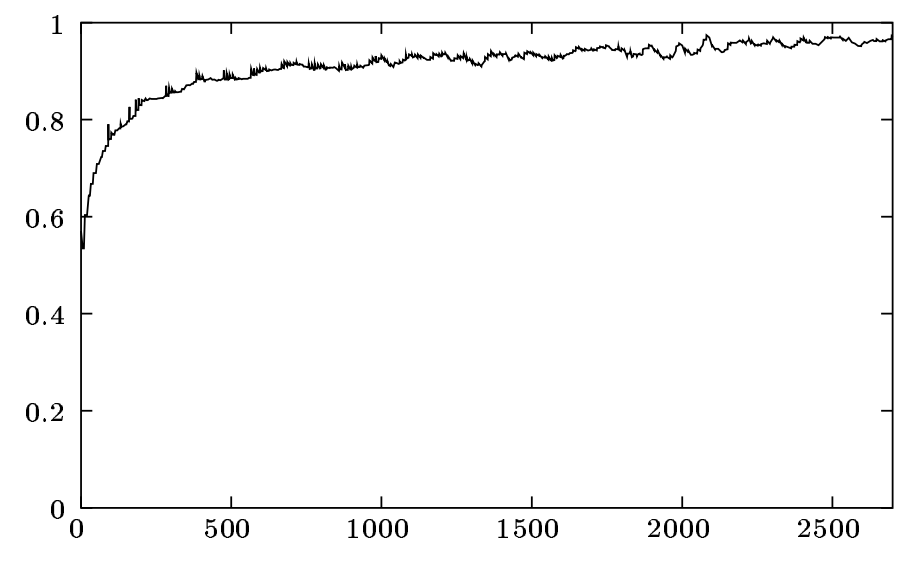
\includegraphics[width=.6\textwidth]{images/uptime.png}
\caption{Probability of remaining online an additional hour as a function of
uptime.
The $x$ axis represents minutes. The $y$ axis shows the fraction of nodes
that stayed online at least $x$ minutes that also stayed online at least
$x+60$ minutes. Source: Maymounkov {\em et al.} \cite{kad}}
\label{fig:kad-uptime}
\end{figure}

See section \ref{sec:RS-sim} and Blake {\em et al.} \cite{pick2-churn} for a
discussion of how repair bandwidth varies as a function of node churn.

\section{Latency}

Decentralized storage systems can potentially capitalize on
massive opportunities for parallelism.
Some of these opportunities include increased transfer rates, processing
capabilities, and overall throughput even when individual
network links are slow. However, parallelism cannot, by itself, improve {\em
latency}. If an individual network link is utilized as part of an operation,
its latency will be the lower bound for the overall operation.
Therefore, any distributed system
intended for high performance applications must continuously and aggressively
optimize for low latency not only on an individual process scale but also for
the system's entire architecture.

\section{Bandwidth}\label{sec:req-bandwidth}

Global bandwidth availability is increasing year after year. Unfortunately,
access to
high-bandwidth internet connections is unevenly distributed across the world.
While some users can easily access symmetric, high-speed, unlimited bandwidth
connections, others have significant difficulty obtaining the same type of
access.

In the United States and other countries,
the method in which many residential internet service providers (ISPs)
operate presents two specific challenges for designers of a
decentralized network protocol. The first challenge is
the asymmetric internet connections offered by ISPs.
Customers subscribe to internet service
based on an advertised download speed, but the upload speed is potentially an
order of magnitude or two slower. The second challenge is that bandwidth is
sometimes ``capped'' by the ISP at a fixed amount of allowed traffic per month.
For example, in many
US markets, the ISP Comcast imposes a one terabyte per month bandwidth cap
with stiff fines for customers who go over this limit \cite{comcast-cap}.
An internet connection with a cap of 1 TB/month cannot average more than
385 KB/s over the month without exceeding the monthly bandwidth allowance,
even if the ISP advertises speeds of 10 MB/s or higher.
Such caps impose
significant limitations on the bandwidth available to the network
at any given moment.

With device failure and churn guaranteed, any decentralized system will have a
corresponding amount of repair traffic. As a result, it is important to account
for the bandwidth required not only for data storage and retrieval but also
for data maintenance and repair \cite{pick2-churn}. Designing a
storage system that is careless with bandwidth usage would not only give undue
preference to storage node operators with access to unlimited high-speed
bandwidth but also centralize the system to some degree. In order to keep the storage
system as decentralized as possible and working in as many environments
as possible, bandwidth usage must be aggressively minimized.

Please see section \ref{sec:bandwidth-space-limits} for a discussion on how
bandwidth availability and repair traffic limit usable space.

\section{Object size}

We can broadly classify large storage systems into two groups by average
object size. To differentiate between the two groups, we classify a ``large'' file as a
few megabytes or greater in size. A database is the
preferred solution for storing many small pieces of information,
whereas an object store or filesystem is ideal for storing many large files.

The initial product offering by Storj Labs is designed to function primarily as
a decentralized object store for larger files.
While future improvements may enable
database-like use cases, object storage is the predominant use case described in
this paper. We made protocol design decisions with the assumption that the
vast majority of stored objects will be 4MB or larger. While smaller files are
supported, they may simply be more costly.

It is worth noting that this will not negatively impact use cases that
require reading lots of files smaller than a megabyte. Users can address this
with a packing strategy by aggregating and storing many small files as one
large file.
The protocol supports seeking and streaming, which will allow users to download small files
without requiring full retrieval of the aggregated object.

\section{Byzantine fault tolerance}

Unlike centralized solutions like Amazon S3, Storj operates in an untrusted
environment where individual storage providers are not necessarily assumed to be
trustworthy. Storj operates over the public internet, allowing anyone to sign
up to become a storage provider.

We adopt the Byzantine, Altruistic, Rational (BAR) model \cite{bar} to discuss
participants in the network.

\begin{itemize}
\item {\em Byzantine} nodes may deviate arbitrarily from the suggested
  protocol for any reason. Some examples include nodes that are broken or nodes
  that are actively trying to sabotage the protocol. In general, a
  {\em Byzantine} node is a bad actor, or one that optimizes for a utility
  function that is independent of the one given for the suggested protocol.
\item Inevitable hardware failures aside, {\em Altruistic} nodes are good
  actors and participate in a proposed protocol even if the rational choice is
  to deviate.
\item {\em Rational} nodes are neutral actors and participate or deviate only
  when it is in their net best interest.
\end{itemize}

Some distributed storage systems (e.g. datacenter-based cloud object storage systems)
operate in an environment
where all nodes are considered {\em altruistic}. For example, sans hardware failure
or security breaches, Amazon's storage nodes
will not do anything besides what they were explicitly programmed to do,
because Amazon owns and runs all of them.

In contrast, Storj operates in an environment where every node is
managed by its own independent operator.
In this environment, we can expect that a majority
of storage nodes are {\em rational} and a minority are {\em byzantine}. Storj assumes no
{\em altruistic} nodes.

We must include incentives that encourage the network to ensure that the
rational nodes on the network (the majority of operators) behave as similarly
as possible to the expected behavior of altruistic nodes.
Likewise, incentives that allow for or encourage byzantine behavior must
be eliminated.

\section{Coordination avoidance}\label{sec:coordination-avoidance}

A growing body of distributed database research shows that systems that
avoid coordination wherever possible have far better throughput than systems
where subcomponents are forced to coordinate to achieve correctness
\cite{cap1, cap2, consistency-vs-latency, hat, i-confluence, anna,
calm1, calm2}.
We use Bailis {\em et al.}'s informal definition
that coordination is the requirement that concurrently executing operations
synchronously communicate or otherwise stall in order to complete
\cite{i-confluence}.
This observation happens at all scales and applies not only to distributed
networks but also to
concurrent threads of execution coordinating within the same computer.
As soon as coordination is needed, actors in the system will need to wait for
other actors, and waiting---due to coordination issues---can have a significant
cost.

While many types of operations in a network may require coordination
(e.g., operations that require linearizability\footnote{
Linearizable operations are atomic operations on a specific object where
the order of operations is equivalent to the order given original ``wall clock''
time.
}
\cite{jepsen-consistency, hat, vv-consistency}), choosing strategies that
avoid coordination (such as Highly Available Transactions \cite{hat}) can offer
performance gains of two to three orders of magnitude over wide area networks.
In fact, by carefully avoiding coordination as much as possible, the Anna
database is able to be 10 times faster than both Cassandra and Redis in their
corresponding environments and 700 to 800 times faster than
performance-focused in-memory databases such as Masstree or Intel's TBB
\cite{anna, anna-announce}.
Not all coordination can be avoided, but new frameworks (such as Invariant
Confluence \cite{i-confluence} or the CALM principle \cite{calm1, calm2})
allow system architects to understand when coordination is required for
consistency and correctness. As evidenced
by Anna's performance successes, it is most efficient to avoid coordination
where possible.

Systems that minimize coordination are
much better at scaling from small
to large workloads. Adding more resources to a coordination-avoidant system
will directly increase throughput and performance. However,
adding more resources to a coordination-dependent system
(such as Bitcoin \cite{bitcoin} or even Raft \cite{raft}) will not result in
much additional throughput or overall performance.

To get to exabyte scale, minimizing coordination is one of the key components
of our strategy.
Surprisingly, many decentralized storage platforms are working towards
architectures that require significant amounts of coordination,
where most if not all operations must be accounted for by a single global
ledger. For us to achieve exabyte scale, it is a fundamental requirement to
limit hotpath coordination domains to small spheres which are entirely
controllable by each user.
This limits the applicability of blockchain-like solutions for our use case.

\chapter{Framework}\label{chap:framework}

After having considered our design constraints, this chapter outlines the
design of a framework consisting of only the most fundamental components.
The framework describes
all of the components that must exist to satisfy our constraints.
As long as our design constraints remain constant, this framework will, as
much as is feasible, describe Storj both now and 10 years from now.
While there will be some design freedom within the framework,
this framework will obviate the need for future rearchitectures entirely, as
independent components will be able to be replaced without affecting other
components.

\section{Framework overview}

All designs within our framework will do the following things:

\begin{description}

\item[Store data] When data is stored with the network, a client encrypts
and breaks it up into multiple pieces. The pieces are distributed
to peers across the network. When this occurs, metadata is generated that
contains information on where to find the data again.

\item[Retrieve data] When data is retrieved from the network,
the client will first reference the metadata to identify the locations of the
previously stored pieces.
Then the pieces will be retrieved and the original data will be reassembled
on the client's local machine.

\item[Maintain data] When the amount of redundancy drops below a certain
threshold, the necessary data for the missing pieces is regenerated and
replaced.

\item[Pay for usage] A unit of value should be sent in exchange for
services rendered.

\end{description}

To improve understandability, we break up the design into a collection of eight
independent components and then combine them to form the desired framework.

The individual components are:

\begin{enumerate}
\item Storage nodes
\item Peer-to-peer communication and discovery
\item Redundancy
\item Metadata
\item Encryption
\item Audits and reputation
\item Data repair
\item Payments
\end{enumerate}

\section{Storage nodes}

The storage node's role is to store and return data.
Aside from reliably storing data, nodes should provide
network bandwidth and appropriate responsiveness.
Storage nodes are selected to store data based on various criteria: ping time,
latency, throughput, bandwidth caps, sufficient disk space,
geographic location, uptime, history of responding accurately to audits, and
so forth. In return for their service, nodes are paid.

Because storage
nodes are selected via changing variables external to the protocol, node
selection is an explicit, non-deterministic process in our framework. This means
that we must keep track of which nodes were selected for each upload via a
small amount of metadata; we can't select nodes for storing data implicitly or
deterministically as in a system like Dynamo \cite{dynamo}. As with Lustre
\cite{lustre}, this decision
implies the requirement of a metadata storage system to keep track
of selected nodes (see section \ref{sec:framework-metadata}).

\section{Peer-to-peer communication and discovery}

All peers on the network communicate via a standarized protocol. The
framework requires that this protocol:

\begin{itemize}
\item provides peer reachability, even in the face of firewalls
and NATs where possible.
This may require techniques like STUN \cite{stun}, UPnP \cite{upnp},
NAT-PMP \cite{natpmp}, etc.
\item provides authentication as in S/Kademlia \cite{skad},
where each participant cryptographically
proves the identity of the peer with whom they are speaking to avoid
man-in-the-middle attacks.
\item provides complete privacy. In cases such as bandwidth measurement
(see section \ref{baer}), the client and storage node must be able
to communicate without any risk of eavesdroppers. The protocol should
ensure that all communications are private by default.
\end{itemize}

Additionally, the framework requires a way to look up peer network addresses
by a unique identifier so that, given a peer's network address, any other
peer can connect to it. This responsibility is similar to the internet's
standard domain name system (DNS) \cite{dns},
which is a mapping of an identifier to an
ephemeral connection address, but unlike DNS, there can be no centralized
registration process.
To achieve this, a network overlay, such as Chord \cite{chord},
Pastry \cite{pastry}, or Kademlia \cite{kad}, can be
built on top of our chosen peer-to-peer communication protocol.
See Section \ref{sec:concrete-node-discovery} for
implementation details.

\section{Redundancy}\label{sec:framework-redundancy}

We assume that at any moment, any storage node could go offline permanently.
Our redundancy
strategy must store data in a way that provides access to the data with high
probability, even though any given number of individual nodes may be in
an offline state. To
achieve a specific level of {\em durability} (defined as the probability that
data remains available in the face of failures), many products in this space use
simple replication. Unfortunately, this ties durability to the network {\em
expansion factor}, which is the storage overhead for reliably storing data. This
significantly increases the total cost relative to the stored data.

For example, suppose a certain desired level of durability requires a
replication strategy that makes eight copies of the data. This yields an
expansion factor of 8x, or 800\%. This data then needs to be stored on the
network, using bandwidth in the process. Thus, more replication results in more
bandwidth usage for a fixed amount of data. As discussed in the protocol design
constraints (section \ref{sec:req-bandwidth}) and Blake {\em et al.}
\cite{pick2-churn},
high bandwidth usage prevents scaling, so this is an undesirable
strategy for ensuring a high degree of file durability.

As an alternative to simple replication, {\em erasure codes} provide a much
more efficient method to achieve redundancy.
Erasure codes are well-established in use for both distributed and peer-to-peer
storage systems \cite{p2p-lazy, storj-v2, rs-cd, rs-intro, rs-stragglers, hail,
filefec-packing}.
Erasure codes are an encoding scheme for manipulating
data durability without tying it to bandwidth usage, and have been found to
improve repair traffic significantly over replication \cite{pick2-churn}.
Importantly, they allow changes in durability without changes in expansion
factor.

An erasure code is often described by two numbers, $k$ and $n$. If a block of
data is encoded with a $(k,n)$ erasure code, there are $n$ total generated {\em
erasure shares}, where only any $k$ of them are required to recover the original
block of data. If a block of data is $s$ bytes, each of the $n$ erasure shares
is roughly $s/k$ bytes. Besides the case when $k=1$ (replication), all erasure
shares are unique.

Interestingly, the durability of a $(k=20,n=40)$ erasure code
is better than a $(k=10,n=20)$ erasure code, even though the expansion factor
(2x) is the same for both. This is because the risk is spread
across more nodes in the $(k=20,n=40)$ case. These considerations make erasure
codes an important part of our general framework.

To better understand how erasure codes increase durability without
increasing expansion factors, the following table shows various choices of
$k$ and $n$, along with the expansion factor and associated durability:

\begin{center}
\begin{tabular}{c c c l}
$k$ & $n$ & Exp. factor & P(D) \\ \hline
2 & 4 & 2 & 99.207366813274616\%\\
4 & 8 & 2 & 99.858868985411326\%\\
8 & 16 & 2 & 99.995462406878260\%\\
16 & 32 & 2 & 99.999994620652776\%\\
20 & 40 & 2 & 99.999999807694154\%\\
32 & 64 & 2 & 99.999999999990544\%\\
\end{tabular}
\end{center}

To see how this table was calculated, we'll start
with the simplifying assumption that $p$ is the monthly node
churn rate (that is, the fraction of nodes that will go offline in a month on
average). Mathematically, time-dependent processes are modeled according to
the Poisson distribution, where it is assumed that $\lambda$ events are
observed in the given unit of time.
As a result, we model durability
as the cumulative distribution function (CDF) of the Poisson distribution with mean $\lambda=pn$,
where we expect $\lambda$ pieces of the file to be lost monthly.
To estimate
durability, we consider the CDF up to $n-k$,
looking at the probability that at most $n-k$ pieces
of the file are lost in a month and the file can still be rebuilt.
The CDF is given by:
\begin{align*}
 && P(D) = e^{-\lambda} \sum_{i=0}^{n-k} \frac{\lambda^i}{i!} &&
\end{align*}

The expansion factor still plays a big role in durability, as seen in the
following table:

\begin{center}
\begin{tabular}{c c c l}
$k$ & $n$ & Exp. factor & P(D) \\ \hline
4 & 6 & 1.5 & 97.688471224736705\%\\
4 & 12 & 3 & 99.999514117129605\%\\
20 & 30 & 1.5 & 99.970766304935266\%\\
20 & 50 & 2.5 & 99.999999999999548\%\\
100 & 150 & 1.5 & 99.999999999973570\%\\
\end{tabular}
\end{center}

By being able to tweak the durability independently of the expansion factor,
erasure coding allows very high durability to be achieved with surprisingly
low expansion factors.
Because of how limited bandwidth is as a resource, completely eliminating
replication as a
strategy and using erasure codes only for redundancy causes a drastic
decrease in bandwidth footprint.

Erasure coding also results in storage nodes getting paid more.
High expansion factors dilute the incoming funds per byte across more storage
nodes; therefore, low expansion factors, such as those provided by erasure
coding, allow for a much more direct passthrough of income to storage node
operators.

\subsection{Erasure codes' effect on streaming}

Erasure codes are used in many streaming contexts such as audio CDs and
satellite communications \cite{rs-cd},
so it's important to point out that using erasure coding in general does not
make our streaming design requirement (required by Amazon S3 compatibility,
see section \ref{constraint-amazon}) more challenging.
Whatever erasure code is chosen for our framework, as with CDs, streaming can
be added on top by encoding small portions at a time, instead of attempting to
encode a file all at once. See section \ref{sec:structured-file-storage} for
more details.

\subsection{Erasure codes' effect on long tails}\label{sec:long-tail}

Erasure codes enable an enormous performance benefit, which is the ability to
avoid waiting for ``long-tail'' response times \cite{tail-at-scale}. A
long-tail response occurs in situations where a needed server has an
unreasonably slow operation time due to a confluence of unpredictable factors.
Long-tail responses are so-named due to their rare average rate of occurrence
but highly variable nature, which in a probability density graph looks like a
``long tail.''
In aggregate, long-tail responses are a big issue in distributed system design.

In MapReduce, long-tail responses are called ``stragglers.''
MapReduce executes redundant requests called ``backup tasks'' to make
sure that if specific stragglers take too long, the overall operation can still
proceed without waiting. If the backup task mechanism is disabled in MapReduce,
basic operations can take 44\% longer to complete, even though
the backup task mechanism is causing duplicated work \cite{mapreduce}.

By using erasure codes, we are in a position to create MapReduce-like
backup tasks for storage \cite{rs-stragglers, rs-intro}.
For uploads, a file can be encoded to a higher $(k, n)$ ratio than
necessary for desired durability guarantees.
During an upload, after enough pieces have uploaded to gain required
redundancy, the remaining additional uploads can be canceled.
This cancellation allows the upload to continue as fast as the fastest nodes
in a set, instead of waiting for the slowest nodes.

\begin{figure}[!htbp]
\centering
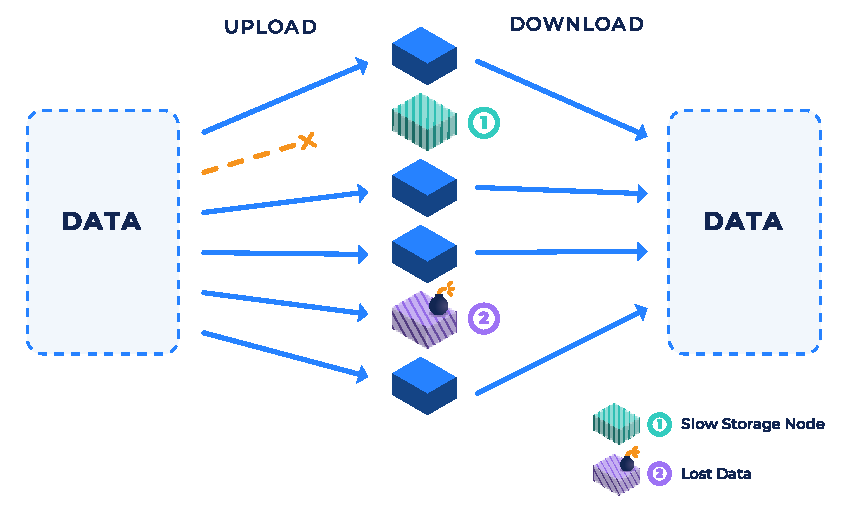
\includegraphics[height=.35\textheight]{images/redundancy.eps}
\caption{Various outcomes during upload and download}
\end{figure}

Downloads are similarly improved. Since more redundancy exists than is needed,
downloads can be served from the fastest peers, eliminating a wait for temporarily slow or offline peers.

The outcome is that every request is satisfiable by the fastest nodes
participating in any given transaction, without needing to wait for a slower
subset.
Focusing on operations where the result is only dependent on the fastest
nodes of a random subpopulation turns what could be a potential liability
(highly variable performance from individual actors) into a great source of
strength for a distributed storage network, while still providing great load
balancing characteristics.

This ability to over-encode a file greatly assists dynamic load balancing of
popular content on the network. See section \ref{sec:future-hot-files} for
a discussion on how we plan to address load balancing very active files.

\section{Metadata}\label{sec:framework-metadata}

Once we split an object up with erasure codes and select storage nodes on
which to store the new pieces, we now need to keep track of which storage
nodes we selected. We allow users to choose storage based on geographic
location, performance characteristics, available space, and other features.
Therefore, instead of implicit node selection such as a scheme using consistent
hashing like Dynamo \cite{dynamo}, we must use an explicit node selection
scheme such as directory-based lookups \cite{p2p-policies}.
Additionally, to maintain Amazon S3 compatibility, the user must be able to
choose an arbitrary key, often treated like a path, to identify this mapping
of data pieces to node. These features imply the necessity of a metadata
storage system.

Amazon S3 compatibility once again imposes some tight requirements.
We should support:
hierarchical objects (paths with prefixes), per-object key/value storage,
arbitrarily large files, arbitrarily large amounts of files, and so forth.
Objects should be able to be stored and retrieved by arbitrary key; in addition,
deterministic iteration over those keys will be required to allow for
paginated listing.

Every time an
object is added, edited, or removed, one or more entries in this metadata
storage system will need to be adjusted. As a result, there could be heavy churn
in this metadata system, and across the entire userbase the metadata itself
could end up being sizable.

For example, suppose in
a few years the network stores one total exabyte of data, where the average object
size is 50MB and our erasure code is selected such that $n=40$.
One exabyte of 50MB objects is 20 billion objects.
This metadata system will need
to keep track of which 40 nodes were selected for each object.
If each metadata element is roughly $40\cdot 64+192$ bytes (info for each
selected node plus the path and some general overhead), there are over 55
terabytes of metadata of which to keep track.

Fortunately, the metadata can be heavily partitioned by the user. A user storing
100 terabytes of 50 megabyte objects will only incur a metadata overhead of 5.5
gigabytes. It's worth pointing out that these numbers vary
heavily with object size: the larger the average object size, the less the
metadata overhead.

An additional framework focus is enabling this component---metadata
storage---to be interchangeable. Specifically, we expect the platform to incorporate
multiple implementations of metadata storage that users will be allowed to
choose between. This greatly assists with our design goal of coordination
avoidance between users (see section \ref{sec:coordination-avoidance}).

Aside from scale requirements, to implement Amazon S3 compatibility,
the desired API is straightforward and
simple: {\em Put} (store metadata at a given path), {\em Get} (retrieve metadata at a
given a path),
{\em List} (paginated, deterministic listing of existing paths), and {\em Delete}
(remove a path). See figure \ref{fig:s3-api-code} for more details.

\section{Encryption}

Regardless of storage system, our design constraints require total security
and privacy. All data or metadata will be encrypted.
Data should be encrypted as early as possible in the data storage pipeline,
ideally before the data ever leaves the source computer. This means that an
Amazon S3-compatible interface or appropriate similar client library should run
colocated on the same computer as the user's application.

Encryption should use a pluggable mechanism that allows users to choose their
desired encryption scheme. It should also store metadata about that encryption
scheme to allow users to recover their data using the appropriate decryption
mechanism, even when their encryption choices are changed or upgraded.

To support rich access management features, the same encryption key should not
be used for every file, as having access to one file would result in access
to decryption keys for all files. Instead, each file should be encrypted with
a unique key. This should allow users to share access to certain selected files
without giving up encryption details for others.

Because each file should be encrypted differently with different keys and
potentially different algorithms, the metadata about that encryption must
be stored somewhere in a manner that is secure and reliable. This metadata,
along with other metadata about the file, including its path, will
be stored in the previously discussed metadata storage system, encrypted
by a deterministic, hierarchical encryption scheme.
A hierarchical encryption scheme based on
BIP32 \cite{bip32} will allow subtrees to be shared without sharing their
parents and will allow some files to be shared without sharing other files.
See section \ref{sec:concrete-encryption} for a discussion of our path-based
hierarchical deterministic encryption scheme.

\section{Audits and reputation}\label{sec:framework-audits}

Incentivizing storage nodes to accurately store data is of paramount importance
to
the viability of this whole system. It is essential to be able to
validate and verify that storage nodes are accurately storing what they have
been
asked to store.

Many storage systems use probabilistic per-file audits, called
{\em proofs of retrievability}, as a way of determining
when and where to repair files \cite{juels, shacham}.
We are extending the probabilistic nature of common per-file
proofs of retrievability to range across all possible files.
Audits, in this case, are probabilistic challenges that confirm, with a high
degree of certainty and a low amount of overhead, that a storage node is
well-behaved, keeping the data it claims, and not susceptible to hardware
failure or malintent. Audits function as ``spot checks'' \cite{juels2} to help
calculate the future usefulness of a given storage node.

In our storage system,
audits are simply a mechanism used to determine a node's degree of stability.
Failed audits will result in a storage node being marked as bad, which
will result in redistributing data to new nodes and avoiding that node altogether
in the future. Storage node uptime and overall health are the primary metrics
used to determine which files need repair.

As is the case with proofs of retrievability \cite{juels, shacham},
this auditing mechanism does not audit all bytes in all files. This can
leave room for false positives, where the verifier believes the storage node
retains the intact data when it has actually been modified or partially
deleted. Fortunately, the probability of a false positive on an individual
partial audit is easily calculable (see section
\ref{sec:audit-false-positive}). When applied
iteratively to a storage node as a whole, detection of missing or altered data
becomes certain to within a known and modifiable error threshold.

A reputation system is needed to persist the history of audit outcomes for
given node identities. Our overall framework has flexible requirements on the use
of such a system, but see section \ref{sec:concrete-reputation} for a
discussion of our initial approach.

\section{Data repair}

Data loss is an ever-present risk in any distributed storage system. While there
are many potential causes for file loss, storage node churn (storage
nodes joining and leaving the network) is the largest leading risk by a
significant degree compared to other causes.
As discussed in section \ref{sec:constraint-churn}, network session time in
many real world systems range from hours to mere minutes \cite{dht-churn}.
While there are many other ways data might get lost, such as corruption,
malicious behavior, bad hardware, software error, or user initiated space
reclamation, these issues are less serious than full node churn. We expect
node churn to be the dominant cause of data loss in our network.

Because audits are validating that conforming nodes store data correctly, all
that remains is to detect when a storage node stops storing
data correctly or goes offline and then repair the data it had to new nodes.
To repair the data, we will recover the original data via an erasure code
reconstruction from the remaining pieces and then regenerate the missing
pieces and store them back in the network on new storage nodes.

It is vital in our system to incentivize storage node participants to remain
online for much longer than a few hours. To encourage this behavior,
our payment strategy will involve rewarding storage node
operators that keep their nodes participating for months and years at a time.

\section{Payments}

Payments, value attribution, and billing in decentralized networks are a
critical part of maintaining a healthy
ecosystem of both supply and demand. Of course, decentralized payment systems
are still in their infancy in a number of ways.

For our framework to achieve low latency and high throughput, we must not have
transactional dependencies on a blockchain (see section \ref{sec:coordination-avoidance}).
This means that an adequately performant storage system cannot afford to
wait for blockchain operations. When operations should be measured in
milliseconds, waiting for a cluster of nodes to probabilistically come to
agreement on a shared global ledger is a non-starter.

Our framework instead emphasizes game theoretic models to ensure
that participants in the network are properly incentivized to remain in the
network and behave rationally to get paid.
Many of our decisions are modeled after real-world financial relationships.
Payments will be transferred during
a background settlement process in which well-behaved participants within
the network cooperate. Storage nodes in our framework should limit their exposure
to untrusted payers until confidence is gained that those payers are likely
to pay for services rendered.

In addition, the system also tracks and aggregates the value of the
consumption of those services by those who own the data stored on the network.
By charging for usage, the framework is able to support the end-to-end
economics of the storage marketplace ecosystem.

Although the Storj network is payment agnostic and
the protocol does not require a specific payment type,
the network assumes the Ethereum-based STORJ token as the default mechanism
for payment. While we intend for the STORJ token to be the primary form of payment, in the future other alternate payment types could be implemented, including Bitcoin,
Ether, credit or debit card, ACH transfer, or even physical transfer of
live goats.

\chapter{Concrete implementation}\label{chap:concrete}

We believe the framework we've described to be relatively fundamental
given our design constraints. However, within the framework there still remains
some freedom in choosing how to implement each component.

In this section, we lay out our initial implementation strategy. We expect
the details contained within this section to change gradually over time.
However, we believe the details outlined here are viable and support a working
implementation of our framework capable of providing highly secure, performant,
and durable production-grade cloud storage.

As with our previous version \cite{storj-v2}, we will publish changes to this
concrete architecture through our Storj Improvement Proposal process \cite{sips}.

\section{Definitions}

The following defined terms are used throughout the description of the concrete
implementation that follows:

\subsection{Actors}

\begin{description}
\item[Client] A user or application that will upload or download data from the network.

\item[Peer class] A cohesive collection of network services and
  responsibilities. There are three different peer classes that represent
  services in our network: {\em storage nodes}, {\em Satellites}, and {\em Uplinks}.

\item[Storage node] This peer class participates in the node discovery
  system, stores data for others, and gets paid for storage and bandwidth.

\item[Uplink] This peer class represents any application or
  service that implements {\em libuplink} and wants to store and/or retrieve data. This peer class
  is not expected to remain online like the other two classes and is
  relatively lightweight. This peer class performs encryption, erasure encoding,
  and coordinates with the other peer classes on behalf of the customer/client.

  \begin{description}
  \item[libuplink] A library which provides all necessary functions to interact
    with {\em storage nodes} and {\em Satellites} directly. This library will
    be available in a number of different programming languages.

  \item[Gateway] A service which provides a compatibility layer between other
    object storage services such as Amazon S3 and {\em libuplink} exposing an
    Amazon S3-compatible API.

  \item[Uplink CLI] A command line interface for uploading and downloading
    files from the network, managing permissions and sharing, and managing
    accounts.
  \end{description}

\item[Satellite] This peer class participates in the node discovery system,
  caches node address information, stores per-object metadata, maintains storage
  node reputation, aggregates billing data, pays storage nodes, performs audits and repair, and manages
  authorization and user accounts.
  Any user can run their own Satellite, but we expect many users
  to elect to avoid the operational complexity and create an account on
  another Satellite hosted by a trusted third party such as Storj Labs,
  a friend, group, or workplace.

\end{description}

\begin{figure}[!htbp]
\centering
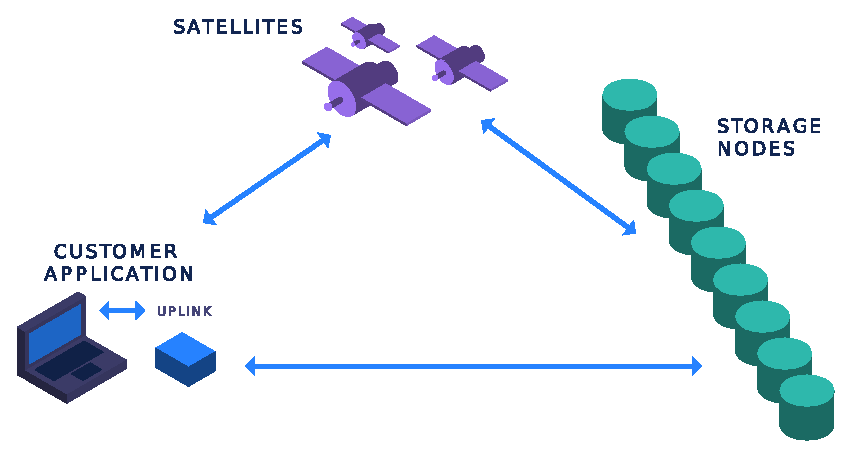
\includegraphics[width=.75\textwidth]{images/overview.eps}
\caption{The three different peer classes}
\end{figure}

\subsection{Data}

%% TODO: hex bytes have lowercase as in them

\begin{figure}[!htbp]
\centering
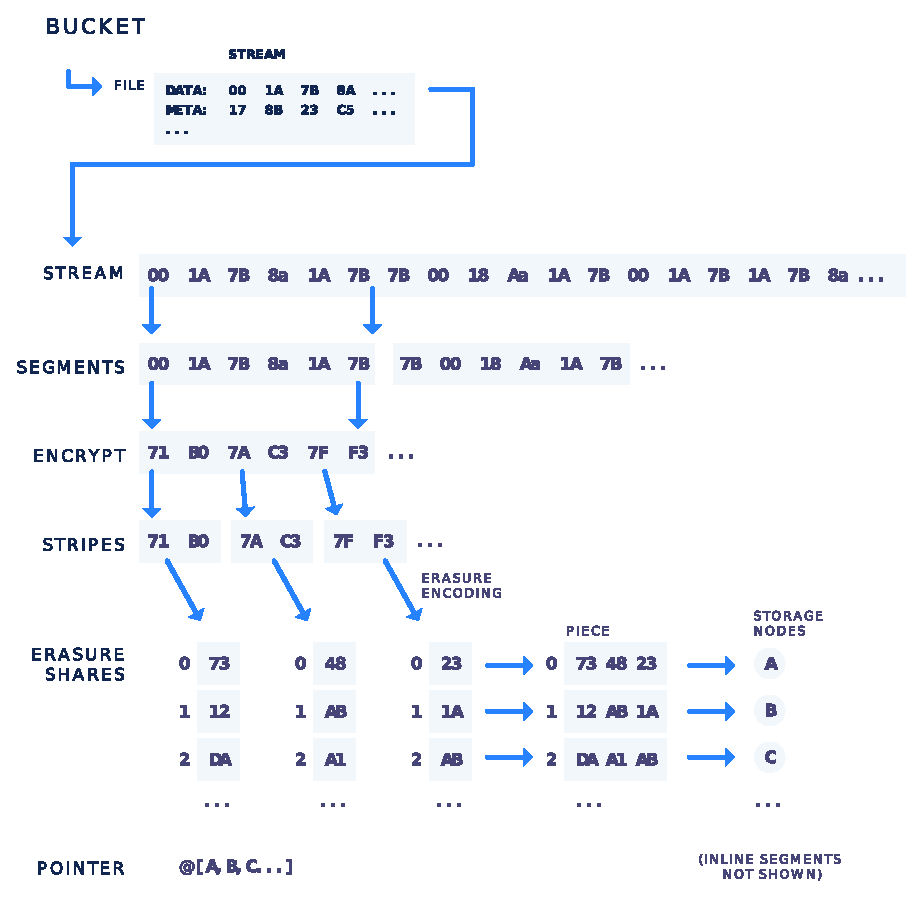
\includegraphics[width=\textwidth]{images/structure.eps}
\caption{Files, segments, stripes, erasure shares, and pieces}
\end{figure}

\begin{description}
\item[Bucket] A {\em bucket} is an unbounded but named collection of files
identified by paths.
Each path represents one file, and every file has a unique path within a bucket.

\item[Path] A {\em path} is a unique identifier for a file within a
bucket. A {\em path} is a string of bytes that begins with a forward
slash byte and ends with something besides a forward slash byte. Forward
slashes (referred to as the path separator) separate non-empty path components.
An example {\em path} might be \code{/etc/hosts}, where the path components are
\code{etc} and \code{hosts}.
Unless otherwise requested,
we encrypt paths before they ever leave the customer's application's
computer.

\item[File or Object] A {\em file} (or {\em object}) is the main data type in
our system. A file is referred to by a path, contains an arbitrary amount of
bytes, and has no minimum or maximum size. A file is represented as an ordered
collection of one or more segments. Segments have a fixed maximum size.
A file also supports a limited amount of key/value user-defined fields
called extended attributes.
Like paths, the data contained in a file is encrypted before it ever
leaves the client computer.

\item[Extended attribute] An {\em extended attribute} is a user defined key/value
field that is associated with a file. Like other per-file metadata,
extended attributes are stored encrypted.

\item[Segment] A {\em segment} represents a single array of bytes, between 0 and a
user-configurable maximum {\em segment} size.
See section \ref{files-as-segments} for more.

\item[Remote Segment] A {\em remote segment} is a segment that will be
encoded and distributed across the network. A {\em remote segment} is larger than
the metadata required to keep track of its bookkeeping, which includes
information such as the IDs of the nodes that the data is stored on.

\item[Inline Segment] An {\em inline segment} is a segment that is small
enough where the data it represents takes less space than the corresponding
data a remote segment will need to keep track of which nodes had the data.
In these cases, the data is stored ``inline'' instead of being stored on nodes.

\item[Stripe] A {\em stripe} is a further subdivision of a segment. A
{\em stripe} is a fixed amount of bytes that is used as an encryption and erasure
encoding boundary size. Erasure encoding happen on {\em stripes} individually;
whereas, encryption may happen on a small multiple of {\em stripes} at a time.
All segments are encrypted, but only remote segments erasure encode stripes.
A {\em stripe} is the unit on which audits are performed.
See section \ref{segments-as-stripes} for more.

\item[Erasure Share] When a stripe is erasure encoded, it generates
multiple pieces called {\em erasure shares}. Only a subset of the {\em erasure
shares} are needed to recover the original stripe. Each {\em erasure
share} has an index identifying which {\em erasure share} it is (e.g., the first,
the second, etc.).

\item[Piece] When a remote segment's stripes are erasure encoded into
erasure shares, the erasure shares for that remote segment with the
same index are concatenated together, and that concatenated group of erasure
shares is called a {\em piece}. If there are $n$ erasure shares after erasure
encoding a stripe, then there are $n$ {\em pieces} after processing a remote
segment. The $i$th {\em piece} is the concatenation of all of the $i$th
erasure shares from that segment's stripes.
See section \ref{erasure-shares-as-pieces} for more.

\item[Pointer] A {\em pointer} is a data structure that either contains the
inline segment data, or keeps track of which
storage nodes the pieces of a remote segment were stored on, along with other
per-file metadata.

\end{description}

\section{Peer classes}

Our overall strategy extends from our previous version \cite{storj-v2} and
also heavily mirrors the Lustre distributed filesystem \cite{lustre}. In
both Lustre and our systems, there are three major actors in the network:
metadata servers, object storage servers, and clients. Object
storage servers hold the bulk of the data stored in the system. Metadata
servers keep track of per-object metadata and where the objects are located
on object storage servers. Clients provide a coherent view and easy access
to files by communicating with both the metadata and object storage servers.

Lustre's architecture is proven for high performance. The majority of the top
100 fastest supercomputers use Lustre for their high-performance, scalable
storage \cite{lustre}. While we don't expect to achieve equal performance over
a wide-area network, we expect dramatically better performance than other
architectures. Any limitation, if any, we experience in performance will be
due to factors besides our overall architecture.

Our previous version used different names for each component. What we
previously referred to as Storj Share, we now refer to as simply storage nodes.
Our formerly centralized single Bridge instance can now be run by anyone and
is referred to as a Satellite.
Our {\em libstorj} library will be made to be backwards
compatible where possible, but we now refer to client software as
Uplinks.

Our network allows these different peer classes and associated functions to be
run separately and independently by different operators, unlike blockchain-based
decentralized storage networks where every node is identical and must perform the
same actions.

\section{Storage node}\label{sec:concrete-storage-nodes}

The main duty of the storage node is to reliably store and return data.
Node operators
are individuals or entities that have excess hard drive space and want to earn
income by renting their space to others. These operators will
download,
install, and configure Storj software locally, with no account required
anywhere.\footnote{Registration with a US-1099 tax form service may be
required. See section \ref{sec:qc}.}
They will then configure disk space and per-Satellite bandwidth allowance.
During node discovery, storage nodes will advertise how much bandwidth and
hard drive space is available, and their designated STORJ token wallet address.

To support Amazon S3 functionality,
storage nodes also keep track of optional per-piece ``time-to-live'', or TTL,
designations.
Pieces may be stored with a specific TTL expiry where data is expected to
be deleted after the expiration date. If no TTL is provided, data is expected
to be stored indefinitely. This means storage nodes have a database of
expiration
times and must occasionally clear out old data.

Storage nodes must additionally keep track of signed bandwidth allocations
(see section \ref{baer}) to send to
Satellites for later settlement and payment. This also requires a small
database. Both TTL and bandwidth allocations are stored in a SQLite
\cite{sqlite} database.

Storage nodes can choose with which Satellites to work. If they work
with multiple Satellites (the default behavior), then payment may come from
multiple sources on varying payment schedules.
Storage nodes are paid by specific Satellites for (1) returning data when
requested in
the form of egress bandwidth payment, and for (2) storing data at rest.
Storage nodes are expected to reliably store all data sent to them and are
paid with the assumption that they are faithfully storing all data.
Storage nodes that fail random audits will be removed from the pool, can lose
funds held in escrow to cover additional costs, and will
receive
limited to no future payments.
Storage nodes are {\em not} paid for the initial transfer of data to store
(ingress bandwidth).
This is to discourage storage nodes from deleting data only to be paid for
storing more, which became a problem with our previous version \cite{storj-v2}.
While storage nodes are paid for repair egress bandwidth usage,
some Satellites may opt to pay less than normal retrieval egress bandwidth
usage.
Storage nodes are not paid for node discovery or any other maintenance traffic.

Storage nodes will support three methods: \code{get}, \code{put}, and
\code{delete}.
Each method will take a {\em piece ID}, a {\em Satellite ID}, a signature
from the associated Satellite instance, and a bandwidth allocation (see
section \ref{baer}).
The {\em Satellite ID} forms a namespace. An identical {\em piece ID} with a
different {\em Satellite ID} refers to a different {\em piece}.

The \code{put} operation will take a stream of bytes and an optional TTL and
store the bytes such
that any subrange of bytes can be retrieved again via a \code{get} operation.
\code{Get} operations are expected to work until the TTL expires (if a TTL was
provided), or until a \code{delete} operation is received, whichever comes
first.
Storage nodes will {\em not} be penalized for rejecting initial \code{put}
operations.

Storage nodes will allow administrators to configure maximum allowed disk
space and per-Satellite bandwidth usage over the last rolling 30 days.
They will keep track of how much is remaining of both, and reject operations
that do not have a valid signature from the appropriate Satellite.

The storage node has been developed and released as open source software.

\section{Node identity}\label{sec:node-id}

During setup, storage nodes, Satellites, and Uplinks all generate their own
identity and certificates for use in the network.
This node ID is used for node discovery and routing.

Each node will operate its own certificate authority, which requires a
public/private key pair and a self-signed certificate. The certificate
authority's private key will ideally be kept in cold storage to prevent key
compromise.
It's important that the certificate authority private key be managed with good
operational security because key rotation for the certificate authority will
require a brand new node ID.

\begin{figure}[!htbp]
\centering
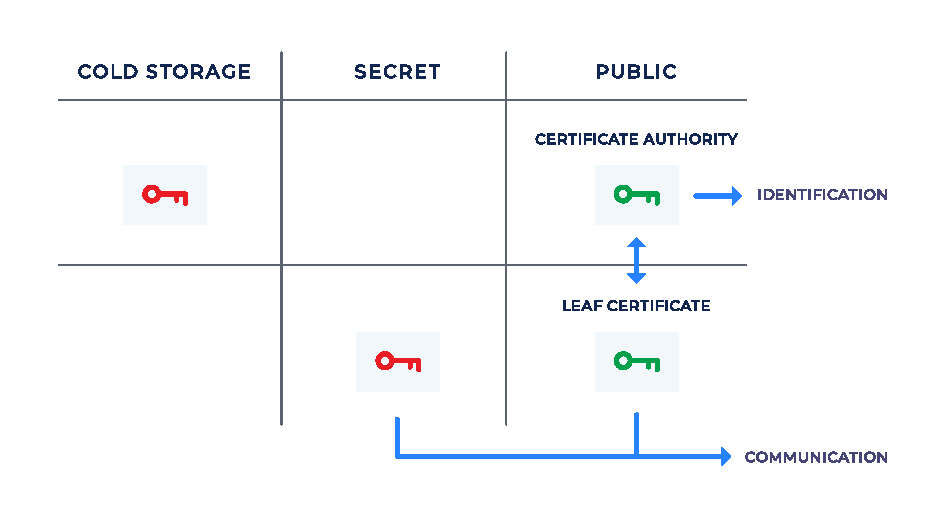
\includegraphics[width=.8\textwidth]{images/identity.eps}
\caption{The different keys and certificates that compose a storage node's
overall identity. Each row represents a private/public key pair.}
\end{figure}

The public key of the node's certificate authority determines its {\em node ID}.
As in S/Kademlia \cite{skad}, the node ID will be the hash of the public key
and will serve as a proof of work for joining the network. Unlike Bitcoin's
proof of work \cite{bitcoin}, the proof of work will be dependent on how many
{\em trailing}
zero bits one can find in the hash output. This means that the node ID (which
may end with a number of trailing zero bits) will
still be usable in a balanced Kademlia \cite{kad} tree.
This cost is meant to make Sybil attacks prohibitively expensive and time
consuming.

Each node will have a revocable leaf certificate and key pair that is signed by
the node's certificate authority. Nodes use the leaf key pair for
communication. Each leaf has a signed timestamp that Satellites
keep track of per node. Should the leaf become compromised, the node can issue
a new leaf with a later timestamp. Interested peers will make note of newly
seen leaf timestamps and reject connections from nodes with older leaf
certificates. As an optimized special case, peers will not need to make a note
when the leaf certificate and certificate authority share the same timestamp.

\section{Peer-to-peer communication}

Initially, we are using the gRPC \cite{grpc} protocol on top of of the
Transport Layer Security protocol (TLS) \cite{tls} on top of the $\mu$TP
\cite{utp} transport protocol with added Session Traversal Utilities for NAT
(STUN) functionality \cite{stun}.
STUN provides NAT traversal; $\mu$TP provides reliable,
ordered delivery (like TCP would); TLS provides privacy and authentication;
and gRPC provides multiplexing and a convenient programmer interface.
Over time, we will replace TLS with a more flexible secure transport
framework (such as the Noise Protocol Framework \cite{noise-proto}) to
reduce round trips due to connection handshakes in situations where the data is
already encrypted and forward secrecy isn't necessary.

When using authenticated communication such as TLS or Noise, every peer can
ascertain the ID of the node with which it is
speaking by validating the certificate chain and hashing its peer's
certificate authority's public key. It can then be estimated how much work went
into constructing the node ID by considering the number of trailing zero bits
at the end of the ID.
Satellites can configure a minimum proof of work required to pass an
audit (section \ref{sec:concrete-audits}
such that, over time, the network will require greater proofs of work
due to natural user intervention.

For the few cases where a node cannot achieve a successful connection through a
NAT or firewall (via STUN \cite{stun}, uPnP \cite{upnp}, NATPmP \cite{natpmp},
or similar techniques), manual
intervention and port forwarding will be required. In the future, nodes unable
to create a connection through their firewalls may rely on traffic proxying from
other, more available nodes, for a fee. Nodes can also provide
assistance to other nodes for initial STUN setup, public address validation,
and so forth.

\section{Node discovery}\label{sec:concrete-node-discovery}

At this point, we have storage nodes and we have a means to identify and
communicate with
them if we know their address. We must account for the fact that storage nodes
will often be on consumer internet connections and behind routers with
constantly changing IP
addresses. Therefore, the node discovery system's goal is to provide a means to look
up a node's latest address by node ID, somewhat similar to the role DNS
provides for the public internet.

The Kademlia distributed hash table (DHT) is a key/value store with a built-in node lookup protocol.
We utilize Kademlia as our primary source of truth for DNS-like
functionality for node lookup, while ignoring the key/value storage aspects of
Kademlia.
Using only Kademlia for node lookup eliminates the need for some other
functionality Kademlia would otherwise require such as owner-based key
republishing, neighbor-based key republishing, storage and retrieval of values,
and so forth. Furthermore, we avoid a number of other known attacks by using the
S/Kademlia \cite{skad} extensions where appropriate.

Unfortunately, DHTs such as Kademlia require multiple network round trips for
many operations, which makes it difficult to achieve millisecond-level
response times. To solve this problem, we add a basic decentralized caching
service on top of Kademlia.

The caching service will live independently in each Satellite and
attempt to talk to every storage node in the network
on an ongoing basis, perhaps once per hour.
The caching service will then cache
the last known good address for each node, and evict nodes that it hasn't talked
to after a certain period of time.
Storage nodes will not need to be extended to know about these caching services.
We expect this to scale for the
reasonable future, as ping operations are inexpensive, but admit a new solution
may ultimately be necessary.
Fortunately, space requirements are negligible. For instance, caching addresses
for a network of 80k nodes
can be done with only 5MB of memory.\footnote{
This is assuming an ordered in-memory list of 4-tuples of node ID (32 bytes),
IP address (16 bytes for IPv6), port (2 bytes), and timestamp (4 bytes).
$80000\cdot(32 \mbox{B}+16 \mbox{B}+2 \mbox{B}+4 \mbox{B}) \approx 4.12 \mbox{MB}$
}

Based on this design, each Satellite's cache will not be expected to be a primary source
of truth, and results in the cache may be stale. However, due to our redundant
storage strategy, the storage network will be resilient against an expected
degree of node churn and staleness.
Therefore, the system will be robust even if some lookups in the cache
fail or return incorrect addresses.
Furthermore, because our peer-to-peer communication
system already provides peer authentication, a node discovery cache that
sometimes returns faulty
or deliberately misleading address lookup responses can only cause a
loss of performance but not correctness.

Even though the Satellite caches are not the primary source of truth, because repair
(section \ref{sec:concrete-data-repair}) requires rapid determination of
whether a node is online or offline, lookups in our system will stop with the
cache lookup and will not attempt a lookup using Kademlia.
Only after cases of failed audit requests will a fallback, nonconcurrent
lookup in Kademlia
be performed to correct for potentially stale cache information.

In addition to being included in every Satellite,
we plan to host and help set up some well-known community-run node discovery caches.
These caches will perform the duty of quickly returning address information
for a given node ID if the node has been online recently.

With each Kademlia message shared on the network, nodes will include their
available disk space, per-Satellite bandwidth availability,
STORJ wallet address, and any other metadata the network needs.
The node discovery cache will collect this information provided by the nodes,
allowing faster lookups for it as well.

\section{Redundancy}\label{sec:concrete-redundancy}

We use the Reed-Solomon erasure code \cite{rs}.
To implement our solution for reducing the effects of long-tails (see section
\ref{sec:long-tail}), for each object that we store
we choose 4 numbers, $k$, $m$, $o$, and $n$, such that $k\le m\le o\le n$.
The standard Reed-Solomon numbers are $k$ and $n$, where $k$ is the minimum
required number of pieces for reconstruction, and $n$ is the total number of
pieces generated during creation.

\begin{figure}[!htbp]
\centering
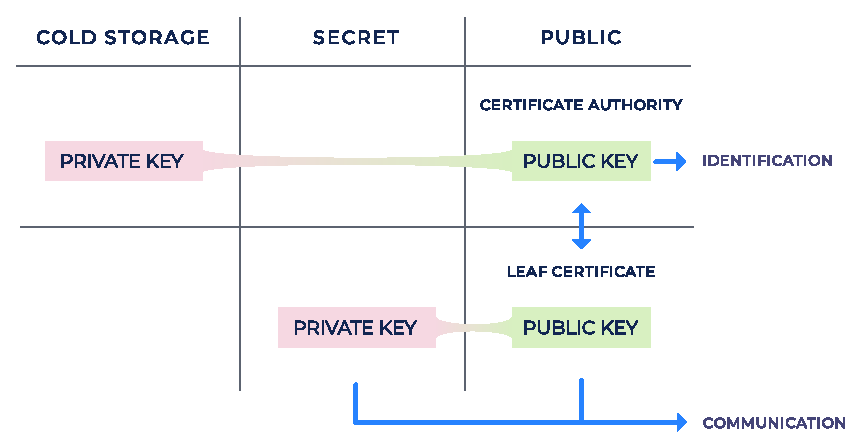
\includegraphics[width=.8\textwidth]{images/kmon.eps}
\caption{The relationship between $k$, $m$, $o$, and $n$.}
\end{figure}

The {\em minimum safe} and {\em optimal} values, respectively, are $m$ and $o$. The
value $m$ is chosen such that if a Satellite notices the amount of available pieces
has fallen below $m$, it triggers a repair
immediately in an attempt to make sure we always maintain
$k$ or more pieces ($m$ is called $r_0$ in Giroire {\em et al.} \cite{p2p-lazy}).
To achieve our long-tail performance improvements
\cite{rs-stragglers, tail-at-scale, mapreduce, rs-intro},
the value $o$ is chosen such that during uploads and repairs,
as soon as $o$ pieces have finished uploading, remaining pieces up to $n$ are
canceled.
Furthermore, $o$ is chosen such that storing $o$ pieces is all that is
needed to achieve the desired durability goals; $n$ is thus chosen such that
storing $n$ pieces will be excess durability.

The amount of long tail uploads we can tolerate is $n-o$, and thus is the amount
of slow nodes to which we are immune.  The amount of nodes that can go
temporarily offline at the same time without triggering a repair is $o-m$. The
safety buffer to avoid losing the data between the time we recognize the data
requires a repair and the actual repair is executed is $m-k$.

See section \ref{sec:RS} for how we select our Reed-Solomon numbers.
Also see section \ref{sec:concrete-data-repair} for a discussion about
how we repair data as its durability drops over time.

\section{Structured file storage}\label{sec:structured-file-storage}

\subsection{Files with extended attributes}

Many applications benefit from being able to keep metadata alongside files.
Amazon S3 supports ``object metadata'' \cite{s3-object-meta} to assist with this
need. This functionality is called ``extended attributes'' in many POSIX
compatible systems, which name we continue using in our system.
Every file will include a limited set of user-specified key-value pairs
(extended attributes) that will be stored alongside other metadata about the
file.

\subsection{Files as Segments}\label{files-as-segments}

\begin{center}
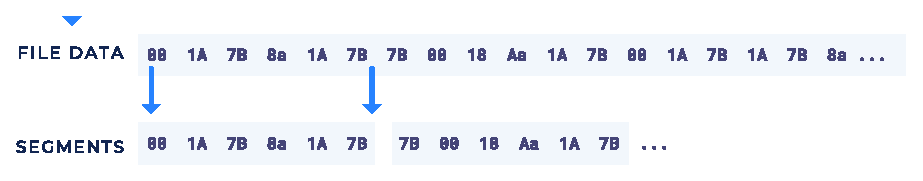
\includegraphics[width=.9\textwidth]{images/stream-segment.eps}
\end{center}

In our previous version \cite{storj-v2}, the term {\em shard} referred to
{\em pieces} on storage nodes, whereas {\em sharding} referred to segmenting a file
into smaller chunks for easier processing. With the addition of erasure coding
in our previous version, these terms became somewhat confusing, so we have
decided to distinguish each meaning with new words.

The sharding process is now called {\em segmenting}, and the highest level
subdivision of a file's stream of data is called a {\em segment}.
Unfortunately, there is general inconsistency using these terms in the
literature. Lustre refers to segments as stripes, but we use the term
{\em stripes} for a further subdelineation \cite{lustre}.

A file may be small enough that it consists of only one segment.
If that segment is smaller than the metadata required to store it on the
network, the data will be stored inline with the metadata.\footnote{
The Linux filesystem Ext4 performs the same optimization
with inline {\em inodes} \cite{ext4-inline}.}
We call this an {\em inline segment}.

For larger files, the data will be broken
into one or more large remote segments. Segmenting in this manner offers
numerous advantages to security, privacy, performance, and availability.
As in Lustre, segmenting large files (e.g. videos) and distributing the segments
across the network reduces the impact of content delivery on any
given node, as
bandwidth demands are distributed more evenly across the network.
As with our previous version \cite{storj-v2},
standardized sizes help frustrate attempts to determine the content of a given
segment and can help obscure the flow of data through the network.
In addition, the end user can take advantage of parallel transfer, similar to
BitTorrent \cite{bittorrent} or other peer-to-peer networks.
Lastly, capping the size of segments
allows for more uniform storage node filling. Thus, a node only needs enough
space to store a segment to participate in the network,
and a client doesn't need
to find nodes that have enough space for a large file.

\subsection{Segments as Stripes}\label{segments-as-stripes}

\begin{center}
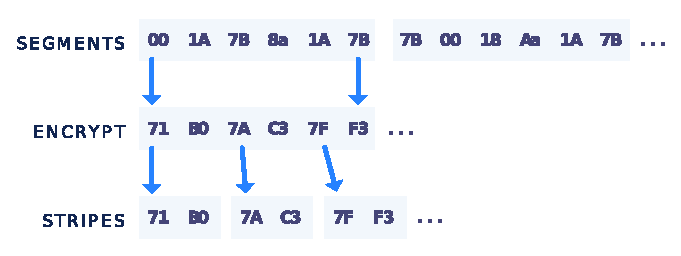
\includegraphics[width=.65\textwidth]{images/segment-stripe.eps}
\end{center}

In many situations, it's important to access a subsection of a larger piece of
data. Some file formats, such as video files or disk images, support seeking,
where only a subset of the data is needed for read operations.
As the creators of audio CDs discovered,
it's useful to be able to decode small parts of a segment
to support these operations \cite{rs-cd}.

A stripe defines a subset of a segment for this purpose and should be no more than a
couple of kilobytes in size. Encryption happens on a small multiple of stripes,
whereas erasure encoding happens on a single stripe at a time. Because we
use authenticated encryption, every encryption batch has a slight overhead,
so slightly larger encryption sizes are preferred. On the other hand, audits
happen on stripes, and we want audit bandwidth usage to be small.

For the reader familiar with the {\em zfec} library, in {\em filefec} mode,
{\em zfec} refers to a stripe as a chunk \cite{filefec-packing}.

\subsection{Stripes as Erasure Shares}\label{stripes-as-erasure-shares}

\begin{center}
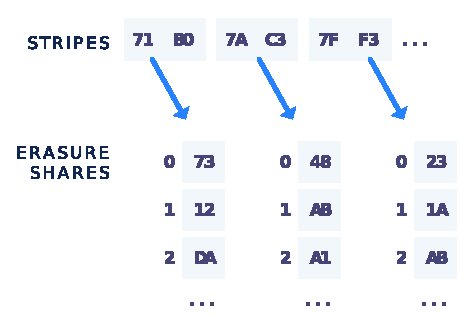
\includegraphics[width=.45\textwidth]{images/stripe-share.eps}
\end{center}

As discussed in sections \ref{sec:framework-redundancy} and
\ref{sec:concrete-redundancy}, erasure codes
give us the chance to control network durability in the face
of unreliable storage nodes.

Stripes are the boundary by which we perform erasure encoding.
In a $(k, n$) erasure code scheme, $n$ erasure shares are generated for
every stripe \cite{rs}.
For example, perhaps a {\em stripe} is broken into 40 {\em erasure shares}
($n=40$), where any 20 ($k=20$) are needed to reconstruct the {\em stripe}. Each
of the 40 {\em erasure shares} will be $1/20$th the size of the original
{\em stripe}.

Erasure encoding
a single stripe at a time allows us to read small portions of a
large segment without retrieving the entire segment first \cite{rs-cd}.
It also allows us to stream data into the
network without staging it beforehand, and it enables a number of other useful
features.

See section \ref{sec:RS-sim} for a breakdown of how varying the erasure code
parameters affects availability and redundancy.

\subsection{Erasure Shares as Pieces}\label{erasure-shares-as-pieces}

\begin{center}
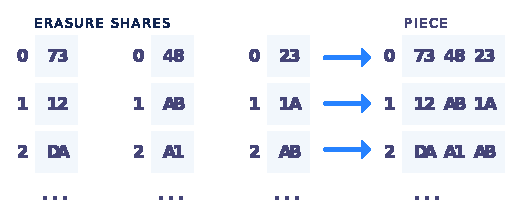
\includegraphics[width=.6\textwidth]{images/share-piece.eps}
\end{center}

Because stripes are already small, erasure shares are often much
smaller, and the metadata to keep track of all of them separately will be
immense relative to their size.
All $n$ erasure shares have a well-defined index associated
with them. More specifically, for
a fixed stripe and any given $n$, the $i$th share of an erasure
code will always be the same.
As with the {\em zfec} library's {\em filefec} mode \cite{filefec-packing},
instead of keeping track of all of the
erasure shares separately, we pack all of the erasure shares with the
same index into a {\em piece}.
In a $(k, n)$ scheme, there are $n$ pieces, where each
piece $i$ is the ordered concatenation of all of the erasure shares with
index $i$. As a result, where each erasure share is $1/k$th of a
{\em stripe}, each piece is $1/k$th of a {\em segment}, and only $k$
pieces are needed to recover the full segment.
A piece is what we store on a storage node.

Satellites generate a brand-new, randomly chosen {\em root piece ID} each time
a new upload begins. The Uplink will keep the {\em root piece ID} secret and send
a {\em node-specific piece ID} to each storage node, formed by taking the Hash-based
Message Authentication Code (HMAC) of the root piece ID and the node's ID.
This serves to obscure what pieces belong together from storage nodes.
The root piece ID is stored in the pointer.

Storage nodes namespace pieces by Satellite ID. If a piece ID used by one
Satellite is reused by another Satellite, each Satellite can safely assume the shared piece ID refers
to a different piece than the other Satellite, with different content and lifecycle.

\subsection{Pointers}

The data owner will need knowledge of how a {\em remote segment} is broken up and
where in the network the {\em pieces} are located to recover it. This is contained
in the {\em pointer} data structure.

A pointer includes: which nodes are storing the pieces,
encryption information, erasure coding details,
the repair threshold amount that determines how much redundancy a segment
must lose before triggering a repair, the amount of pieces that must be
stored to consider a repair to be successful, and other details. If the
segment is an inline segment, the pointer contains the entire segment's binary
data instead of which nodes store the pieces.

In our previous version \cite{storj-v2}, we used two data structures to keep
track of the aforementioned kinds of information:
{\em frames} and {\em pointers}.
In this version we have combined these data structures into a single data
structure and elected to call the new combined data structure a {\em pointer}.

\section{Metadata}\label{sec:concrete-metadata}

The metadata storage system in the Storj network predominantly stores
{\em pointers}. Other individual components of the Storj network communicate with
the pointer database to store and retrieve pointers by path to perform actions.

The most trivial implementation for the metadata storage functionality we
require will be to simply have each user use their preferred trusted database,
such as MongoDB, MariaDB, Couchbase, PostgreSQL, SQLite \cite{sqlite},
Cassandra \cite{cassandra}, Spanner \cite{spanner}, or CockroachDB,
to name a few. In many cases, this will
be acceptable for specific users, provided those users are managing appropriate
backups of their metadata. Indeed, the types of users who have petabytes of data
to store can most likely manage reliable backups of a single relational database
storing only metadata.

There are a few downsides to letting clients manage their metadata in a
traditional database system, such as:
\begin{itemize}
\item {\bf Availability} - The availability of the user's data
is tied entirely to the availability of their metadata server. The counterpoint
is that availability can be made arbitrarily good with existing trusted
distributed solutions, such as Cassandra, Spanner, or CockroachDB, assuming an
appropriate amount of effort put into maintaining operations. Furthermore, any
individual metadata service downtime does not affect the rest of the network. In
fact, the network as a whole can never go down.
\item {\bf Durability} -
If the metadata server suffers a catastrophic failure without backups, all of
the user's data will be lost. This is already true with encryption keys,
but a traditional database solution considerably increases the risk area from just
encryption keys. Fortunately, the metadata itself can be periodically backed
up into the Storj network,
such that only needing to keep track of metadata-metadata
further decreases the amount of critical information that must be stored
elsewhere.
\item {\bf Trust} - The user has to trust the metadata server.
\end{itemize}

On the other hand, there are a few upsides:
\begin{itemize}
\item {\bf Control} - The user is in complete control of all of their data.
  There is no organizational single point of failure. The user is free
  to choose whatever metadata store with whatever trade-offs they prefer and
  can even run their own. Like
  Mastodon\cite{mastodon}, this solution is still decentralized. Furthermore, in a
  catastrophic scenario, this design is no worse than most other technologies or
  techniques application developers frequently use (databases).
\item {\bf Simplicity} - Other projects have spent multiple years on shaky
  implementations of byzantine-fault tolerant consensus metadata storage,
  with expected performance and complexity trade-offs
  (see appendix \ref{chap:dist-consensus}).
  We can get a useful product to market without doing this work at all.
  This is a considerable advantage.
\item {\bf Coordination Avoidance} - Users only need to coordinate with
  other users on their Satellite. If a user has high throughput demands,
  they can set up their own Satellite and avoid coordination overhead from
  any other user. By allowing Satellite operators to select their own database,
  this will allow a user to choose a Satellite with weaker consistency
  semantics, such as Highly Available Transactions \cite{hat}, that reduce
  coordination overhead within their own Satellite and increase performance
  even further.
\end{itemize}

Our launch goal is to allow customers to store their metadata in a database of
their choosing. We expect and look forward to new systems and improvements
specifically in this component of our framework.

Please see appendix \ref{chap:dist-consensus} for more about why we've chosen
to currently avoid trying to solve the problem of Byzantine distributed consensus.
See section \ref{sec:distributed-metadata} for a discussion of future plans.

\section{Satellite}

The collection of services that hold this metadata is called the
{\em Satellite}. Users of the network will have accounts on a specific
Satellite {\em instance}, which will: store their file metadata, manage authorization
to data, keep track of storage node reliability, repair and maintain data when
redundancy is reduced, and issue payments to storage nodes on the user's behalf.
Notably, a specific Satellite instance does not necessarily constitute one
server. A Satellite may be run as a collection of servers and be backed by
a horizontally scalable trusted database for higher uptime.

Storj implements a thin-client model that delegates trust around managing
files' location metadata to the Satellite service which manages data
ownership. {\em Uplinks}
are thus able to support the widest possible array of client applications, while
Satellites require high uptime and potentially significant infrastructure,
especially for an active set of files.
Like storage nodes,
the Satellite service has been developed and released as open source software.
Any individual or organization can run their own Satellite to facilitate
network access.

The Satellite is, at its core, one of the most complex and yet
straightforward components of our initial release that fulfills our framework.
Notwithstanding future framework-conforming releases, the initial Satellite
is a standard application server that wraps a trusted database, such as
PostgreSQL, Cassandra, or whichever solution the metadata system chooses
(section \ref{sec:concrete-metadata}). Users sign in to a specific
Satellite with account credentials.
Data available through one Satellite instance is
not available through another Satellite instance, though various levels of
export and import are planned (section \ref{sec:distributed-metadata}).

With respect to customer data, the Satellite is
never given data unencrypted and does not hold encryption keys.
The only knowledge of an object that the Satellite is able to share with
third parties is its existence, rough size, and other metadata such as access
patterns.
This system protects the client's privacy and gives the client complete
control over access to the data,
while delegating the responsibility of keeping files available on the network
to the Satellite.

Clients may use Satellites run by a third-party. Because Satellites store almost no
data and have no access to keys, this is a large improvement over the
traditional data-center model. Many of the features Satellites provide, like
storage node selection and reputation, leverage considerable network effects.
Reputation data sets grow more useful as they increase in size,
indicating that there are strong economic incentives to share infrastructure
and information in a Satellite.

Providers may choose to operate public Satellites as a service.
Application developers then delegate trust regarding the location of their
data on the network to a specific Satellite, as they
would to a traditional object store but to a lesser degree. Future updates
will allow for various distributions of responsibilities, and thus levels of
trust, between customer applications and Satellites.

The Satellite instance is made up of these components:
\begin{itemize}
\item A full node discovery cache (section \ref{sec:concrete-node-discovery})
\item A per-object metadata database indexed by encrypted path
  (section \ref{sec:concrete-metadata})
\item An account management and authorization system
  (section \ref{sec:concrete-authorization})
\item A storage node reputation, statistics, and auditing system
  (section \ref{sec:concrete-audits})
\item A data repair service (section \ref{sec:concrete-data-repair})
\item A storage node payment service (section \ref{sec:concrete-payments})
\end{itemize}

While our launch goal of many Satellites is a step ahead of our previous
system's Bridge implementation \cite{storj-v2}, this is still just one point on
our decentralization journey and we expect to continue to find ways to
decentralize our components further.
Future releases will see significant improvements to and potentially
rearchitectures of these systems.

\section{Encryption}\label{sec:concrete-encryption}

Our encryption choice is authenticated encryption, with support for both the
AES-GCM cipher and the Salsa20 and Poly1305 combination NaCl calls ``Secretbox''
\cite{nacl-crypto}. Authenticated encryption is used so that the user can know
if anything has tampered with the data.

Data is encrypted in blocks of small batches of stripes, recommended to be
4KB or less \cite{nacl-packetlen}. While the same encryption key is used for
every encryption batch in a segment, segments may have
different encryption keys. However, the nonce for each encryption
batch must be monotonically incrementing from the previous batch throughout the
entire segment. The nonce wraps around to 0 if the counter reaches the
maximum representable nonce.
To prevent reordering attacks, the starting nonce of each
segment is deterministically chosen based on the segment number.
When multiple segments are uploaded in parallel, such as in the case of
Amazon S3's multipart upload feature, the starting nonce for each segment can be
calculated from the starting nonce of the file and the segment number.
This scheme protects the
content of the data from the storage node housing the data. The data owner
retains complete control over the encryption key, and thus over access to the
data.

Paths are also encrypted. Like
BIP32 \cite{bip32}, the encryption is hierarchical and deterministic, and
each path component is encrypted separately. To explain how we do this,
we start with a scheme for determining a secret value for each path
component.
Let's say a given path $\vec{p}$ has path components $p_1, p_2, \ldots, p_n$
and we want to determine an encrypted path $\vec{e}$ with path components
$e_1, e_2, \ldots, e_n$.
We assume a predetermined root secret, $s_0$. This root secret is chosen
by the user and like all other encryption secrets, never leaves the client
computer. We recursively define
$s_i = \mbox{HMAC}(s_{i-1}, p_i)$.
A key can be deterministically generated from $s_i$, $K(s_i)$.
We then define the encrypted path component
$e_i = \mbox{enc}(K(s_{i-1}), p_i)$, such that the new path
$\vec{e}$ is $e_1, e_2, \ldots, e_n$.
HMAC-SHA256 or HMAC-SHA512 are used for key derivations.

This construction allows a client to share access to some subtree of the
path without access to its parents or other paths of the same depth. For
example, suppose a client would like to share access to all paths with the
same prefix $p_1, p_2, p_3$ with another client. The client would give the
other client $e_1, e_2, e_3$ and $s_3$. This allows the client to decrypt
and access any arbitrary $e_4$, as $K(s_3)$ is known to them. More generally
in this case, the client could decrypt and access any arbitrary $e_i$,
where $i > 3$

Path encryption is enabled by default but is otherwise optional, as encrypted
paths make efficient sorted path listing challenging.
When path encryption is in use (a per-bucket feature),
objects are sorted by their encrypted path name, which is deterministic
but otherwise relatively unhelpful
when the client application is interested in sorted, unencrypted paths.
For this reason, users can opt out of
path encryption. When path encryption is disabled, unencrypted paths
are only revealed to the user's chosen Satellite, but not to the storage
nodes. Storage nodes continue to have no information about the path and
metadata of the pieces they store.

\section{Authorization}\label{sec:concrete-authorization}

Encryption protects the privacy of data while allowing for the {\em identification}
of tampering, but authorization allows for the {\em prevention} of tampering by
disallowing clients. Users who are authorized will be able to add, remove,
and edit files, while users who are not authorized will not have those abilities.
Metadata operations will be authorized. Users will authenticate with
their Satellite, which will allow them access to various operations according
to their authorization configuration.

Our initial metadata authorization scheme uses macaroons \cite{macaroons}.
Macaroons are a type of bearer token that authorizes
the bearer to some restricted resources. Macaroons are especially interesting
in that they allow for rich contextual decentralized delegation. Additionally, they
provide the property that anyone can add restrictions in a way in which those
restrictions cannot later be removed.

We use macaroons to restrict which operations can be applied and to which
encrypted paths they can be applied. In this way, macaroons provide a
mechanism to restrict delegated access to specific encrypted path prefixes,
specific files, and specific operations, such as read only access or perhaps
append only access.
Each account has a root macaroon and operations are validated against a supplied
macaroon's set of caveats.
Our macaroons are further caveated with revocation tokens and optional
expirations, which allow users to revoke macaroons programmatically.

Because we want to restrict Satellite operations, and Satellites only have access
to encrypted paths, our authorization scheme must work on encrypted paths. For
access delegation to specific path prefixes, path separation boundaries between
path components must remain across encryption.

Once the Uplink is authorized with the Satellite, the Satellite will approve
and sign for operations to storage nodes, including bandwidth allocations
(section \ref{baer}).
The Uplink must retrieve valid signatures from the Satellite
prior to operations with storage nodes.
All operations on a storage node require a specific Satellite ID and associated
signature.
A storage node will reject operations not signed by the appropriate
Satellite ID. Storage nodes will not allow
operations signed by one Satellite to apply to objects owned by another, unless
explicitly granted by the owning Satellite.

\section{Audits}\label{sec:concrete-audits}

In a network with untrusted nodes, validating that nodes are returning data
accurately and otherwise behaving as expected is vital to ensuring a properly
functioning system. Audits are a way to confirm that nodes have the data they
claim to have. Auditors, such as Satellites, will send a {\em challenge} to a
storage node and expect a valid response. A challenge is a request to the
storage node in order to to prove it has the expected data.

Some distributed storage systems, including the previous version of Storj
\cite{storj-v2}, discuss {\em Merkle tree proofs}, in which audit challenges
and expected responses are generated at the time of storage as a form of
{\em proof of retrievability} \cite{juels}. By using a Merkle tree
\cite{merkle-tree}, the amount of metadata needed to store these
challenges and responses is negligible.

Unfortunately, in such a scheme, the challenges and expected responses must be
pre-generated. As we learned with our previous version, without a periodic
regeneration of these challenges, a storage node can begin to pass most
audits without storing all of the requested data. During our previous version,
we began to consider Reed-Solomon erasure coding to help us solve this problem.

An assumption in our storage system is that most storage nodes are
reasonably well-behaved, and most data is stored faithfully. As long as that
assumption holds, Reed-Solomon is able to detect errors and even correct them,
via mechanisms such as the Berlekamp-Welch error correction algorithm
\cite{bw, rs-intro}.
We are already using Reed-Solomon erasure coding \cite{rs} on small ranges
(stripes), so as discussed in the HAIL system \cite{hail},
we use erasure coding to read a single stripe at a time as a challenge
and then validate the erasure share responses. This allows us to run arbitrary
audits without pre-generated challenges.

To perform an audit, we first choose a stripe. We request that
stripe's erasure shares from all storage nodes responsible. We then run
the Berlekamp-Welch algorithm \cite{bw, rs-intro} across all the
erasure shares. When enough storage nodes return correct information,
any faulty or missing responses can easily be identified.

Given a specific storage node, an audit might reveal that it is offline or
incorrect. In the case of a node being offline, the audit failure
may be due to the address in the node discovery cache being stale, so another,
fresh Kademlia lookup will be attempted. If the node still appears to be offline,
the Satellite places the node in {\em containment} mode. In containment
mode, the Satellite will continue to try the same audit with that node
until the node either responds successfully, actively fails the audit, or
is disqualified from being offline too long. Once the node responds
successfully, it leaves containment mode.
These audit failures will be stored and saved in the reputation system.

It is important that every storage node has a frequent set of random audits to
gain statistical power on how well-behaved that storage node is operating.
However, as discussed in section \ref{sec:framework-audits}, it is
not a requirement that audits are performed on every byte, or even on every
file.

Additionally, it is important that every byte stored in the system has an equal
probability of being checked for a future audit to every other byte in the
system. See section \ref{sec:audit-false-positive} for a discussion on
how many audits are required to be confident data is stored correctly.

\section{Data repair}\label{sec:concrete-data-repair}

As storage nodes go offline---taking their pieces with them---it will
be necessary for the missing pieces to be rebuilt once each segment's pieces
fall below the predetermined threshold $m$. If a node goes offline, the
Satellite will mark that nodes' file pieces as missing.

The node discovery system's caches have reasonably accurate and
up-to-date information about which storage nodes have been online recently.
When a storage node changes state from recently online to offline, this can
trigger a lookup in a reverse index within a user's metadata database,
identifying all segment pointers that were stored on that node.

For every segment that drops below the appropriate minimum safety
threshold, $m$, the segment will be downloaded and reconstructed, and the
missing pieces will be regenerated and uploaded to new nodes. Finally, the
{\em pointer} will be updated to include the new information.

Users will choose their desired durability with their Satellite
which may impact price and other considerations. This desired durability (along with
statistics from ongoing audits) will directly inform what Reed-Solomon erasure
code choices will be made for new and repaired files, and what thresholds
will be set for when uploads are successful and when repair is needed. See
sections \ref{sec:framework-redundancy} and \ref{sec:RS} for how we calculate
these values given user inputs.

A direct implication of this design is that, for now, the Satellite must
constantly stay running. If the user's Satellite stops running, repairs will
stop, and data will eventually disappear from the network due to node churn.
This is similar to the design of how value storing and republishing works in
Kademlia \cite{kad}, which requires the owner to stay online.

The {\em ingress} (or inbound) bandwidth demands of the audit and repair system are large, but
given standard configuration, the {\em egress} (or outbound) demands are relatively small.
A large amount of data comes in to the system for audits and repairs, but only
the formerly missing pieces get sent back out.
While the repair and audit system can run anywhere, the bandwidth usage
asymmetry means that hosting providers which offer free ingress
make for an especially attractive hosting location for users of this system.

\subsection{Piece hashes}\label{sec:concrete-piece-hashes}

Data repair is an ongoing, costly operation that will use significant
bandwidth, memory, and processing power, often impacting a single operator.
As a result, repair resource usage should be aggressively minimized as much as
possible.

For repairing a segment to be effective at minimizing bandwidth usage, as few
pieces as needed for reconstruction should be downloaded. Unfortunately,
Reed-Solomon is insufficient on its own for correcting errors when only a few redundant
pieces are provided. Instead, piece hashes provide a better way to be
confident that we're repairing the data correctly.

To solve this problem, hashes of
every {\em piece} will be stored alongside each piece on each storage node.
A validation hash that the set of hashes is correct will be stored in the
{\em pointer}. During repair, the hashes of every piece can be retrieved and
validated for correctness against the pointer, thus allowing each piece to
be validated in its entirety. This allows the repair system to correctly assess
whether or not repair has been completed successfully without using extra
redundancy for the same task.

\section{Storage node reputation}\label{sec:concrete-reputation}

Reputation metrics on decentralized networks are a critical part of
enabling cooperation
between nodes
where progress would be challenging otherwise. Reputation metrics
are used to ensure that bad actors
within the network are eliminated as participants, improving security,
reliability, and durability.

Storage node reputation can be divided into four subsystems.
The first subsystem is a proof of work identity system,
the second subsystem is the initial vetting process,
the third subsystem is a filtering system, and finally,
the fourth system is a preference system.

The goal of the first system is require a short proof that the storage node
operator is invested, either via time, stake, or resources. We are using
proof of work initially.
As mentioned in section \ref{sec:concrete-storage-nodes}, storage nodes require
a proof of work as part of identity generation. This helps the network avoid
some Sybil attacks \cite{sybil-attack}, but we glossed over how proof of work
difficulty is set. We will let Satellite operators set per-Satellite minimum
difficulty required for new data storage. If a storage node has an identity generated
with a lower difficulty than the Satellite's configured minimum, that storage
node will not be a candidate for new data.
We expect Satellite operators to naturally increase the minimum proof of work
difficulty requirements over time until a reasonable balance is found.
In the case of a changing difficulty configuration, Satellites will leave
existing data on existing nodes where possible.
Other investment proof schemes are possible, such as a form of proof of stake as
we proposed in our previous work \cite{sybil-cost}.

The second subsystem slowly allows nodes to join the network.
When a storage node first joins the network, its reliability is unknown.
As a result, it will be placed into a vetting
process until enough data is known about it.
We propose the following way to gather data about new nodes
without compromising the integrity of the network.
Every time a file is uploaded, the system will select a small number of
additional unvetted storage nodes to include in the list of target nodes.
The Reed-Solomon parameters will be chosen such that these unvetted storage
nodes will not affect the durability of the file, but will allow the network
to test the node
with a small fraction of data until we are sure the node is reliable.
After the storage node has successfully stored enough data for a long enough
period (at least one payment period),
the system will then start including that storage
node in the standard selection process used for general uploads.
Importantly, storage nodes get paid during this
vetting period, but don't receive as much data.

The filtering system is the third subsystem; it blocks bad storage nodes from
participating.
In addition to simply not having done a sufficient proof of work,
certain actions a storage node can take are disqualifying events. The
reputation system will be used to filter these nodes out from future uploads,
regardless of where the node is in the vetting process.
Actions that are disqualifying include: failing too many audits;
failing to return data, with reasonable speed; and failing too many uptime
checks.

If a storage node is disqualified, that node will no longer be selected for
future data storage and the data that node stores will be moved to new
storage nodes.
Likewise, if a client attempts to download a piece from a storage node that
the node should have and the node fails to return it, the
node will be disqualified. Importantly, storage nodes will be allowed to reject
and fail uploads without penalty, as nodes will be allowed to choose which
Satellite operators to work with and which data to store.

It's worth reiterating that failing too many uptime checks is a disqualifying
event. Storage nodes can be taken down for maintenance, but if a storage node
is offline too much, it can have an adverse impact on the network. If a node
is offline during an audit, that specific audit should be retried until the node
responds successfully or is disqualified, to prevent nodes from selectively
failing to respond to audits.

After a storage node is disqualified, the node must go back through the entire
vetting process again. If the node decides to start over with a brand-new
identity, the node must restart the vetting process from the beginning (in
addition to generating a new node ID via the proof of work system). This
strongly disincentivizes storage nodes from being cavalier with their
reputation.

The last subsystem is a preference system. After disqualified storage nodes
have been filtered out, remaining statistics collected during audits
will be used to establish a preference for better storage nodes during uploads.
These statistics include performance characteristics such as throughput and
latency, history of reliability and uptime, geographic location, and other
desirable qualities.
They will be combined into a load-balancing selection process, such
that all uploads are sent to qualified nodes, with a higher likelihood of
uploads to preferred nodes, but with a non-zero chance for any qualified node.
Initially, we'll be load balancing with these preferences via a randomized
scheme, such as the Power of Two Choices \cite{power-of-two-choices}, which
selects two options entirely at random, and then chooses the more qualified
between those two.

On the Storj network, preferential storage node reputation is only used to
select where new data will be stored, both during repair and during the
upload of new files, unlike disqualifying events.
If a storage node's preferential reputation decreases, its file pieces will not
be moved or repaired to other nodes.

There is no process planned in our system for storage nodes to contest their
reputation scores. It is in the best interest of storage nodes to have good
uptime, pass audits, and return data. Storage nodes that don't do these things
are not useful to the network. Storage nodes that are treated by Satellites
unfairly will not accept future data from those Satellites. See section
\ref{sec:qc} about quality control for how we plan to ensure Satellites are
incentivized to treat storage nodes fairly.

Initially, storage node reputation will be individually determined by each
Satellite. If a node is disqualified by one Satellite, it may still
store data for other Satellites. Reputation will not initially be shared between
Satellites. Over time, as we plan to eliminate Satellites,
reputation will then be determined globally.

\section{Payments}\label{sec:concrete-payments}

In the Storj network, payments are made by clients who store data on the
platform to the Satellite they utilize.
The Satellites then pays storage nodes for the amount of storage and bandwidth
they provide on the network.
Payments by clients may be through any mechanism (STORJ, credit card, invoice),
but payments to storage nodes are via the Ethereum ERC20 \cite{erc20} STORJ
token.

Previous distributed systems have handled payments as hard-coded contracts.
For example, the previous Storj network utilized 90-day contracts to maintain
data on the network. After that period of time, the file was deleted.
Other distributed storage platforms use 15-day renewable contracts that delete
data if the user does not login every 15 days. Others use 30-day contracts.
We believe that the most common use case is indefinite storage. To best solve
this use case,
moving forward, our network will not use contracts at all to manage payments
and file storage durations. The default assumption is that data will last
indefinitely.

Satellites will pay storage nodes for the data they store
and for piece downloads.
Storage nodes will not be paid for the initial storage of data, but they
will be paid for storing the data month-by-month. At the end of the payment
period, a Satellite will calculate earnings for each of its storage nodes.
Provided the storage node hasn't been disqualified,
the storage node will be paid by the Satellite for the data it has stored
over the course of
the month, per the Satellite's records.

Satellites have a strong incentive to prefer long-lived storage nodes. If
storage node churn is too high, Satellites will escrow a portion of a storage
node's payment until the storage node has maintained good participation and
uptime for some minimum amount of time, on the order of greater than half a year.
If a storage node leaves the network prematurely, the Satellite will reclaim
escrowed payments to it.

If a storage node misses a delete command due to the node being
offline, it will be storing more data than the Satellite credits it for.
Storage nodes are not paid for storing such file pieces, but
will eventually be cleaned up through the garbage collection process
(see section \ref{sec:garbage-collection}).
This means that storage nodes who maintain higher availability
can maximize their profits by deleting files on request,
which minimizes the amount
of garbage data on their nodes.

The Satellite maintains a database of all file pieces it is responsible for
and the storage nodes it believes are storing these pieces. Each day,
the Satellite adds another day's worth
of credits to each storage node for every file
piece
it will be storing.
Satellites will track utilized bandwidth (see section \ref{baer}).
At the end of the month, each Satellite
adds up all bandwidth and storage payments each storage node has earned and
makes
the payments to the appropriate storage nodes.

Satellites will also earn revenue from account holders for executing audits,
repairing files, and storing metadata. Every day, each Satellite will execute
a number of audits across all of its storage nodes on the network. During an
audit,
if a storage node does not have the file it should be storing, it will
immediately be disqualified and
the Satellite will flag that storage node's file pieces for
repair
in the system.
The Satellite will be paid for both completing the audit
and for the repair,
once that file falls below the file piece threshold needed for
repair.

If a storage node acts
maliciously and does not store files properly or maintain sufficient
availability, it will not be paid for the services rendered, and the funds
allocated to it will instead be used to repair any missing
file pieces and to pay new storage nodes for storing the data.

To reduce transaction fees and other overhead as much as possible, payments
will be recipient-initiated and must be worth at least some minimum value.
Certain Satellites may elect to use a portion of the storage nodes' payout to
cover transaction fees in part or in whole.

See the Satellite reputation section
(section \ref{sec:concrete-satellite-reputation}) for details on
how storage nodes will know to trust Satellites.

\section{Bandwidth allocation}\label{baer}

\begin{figure}[!htbp]
\centering
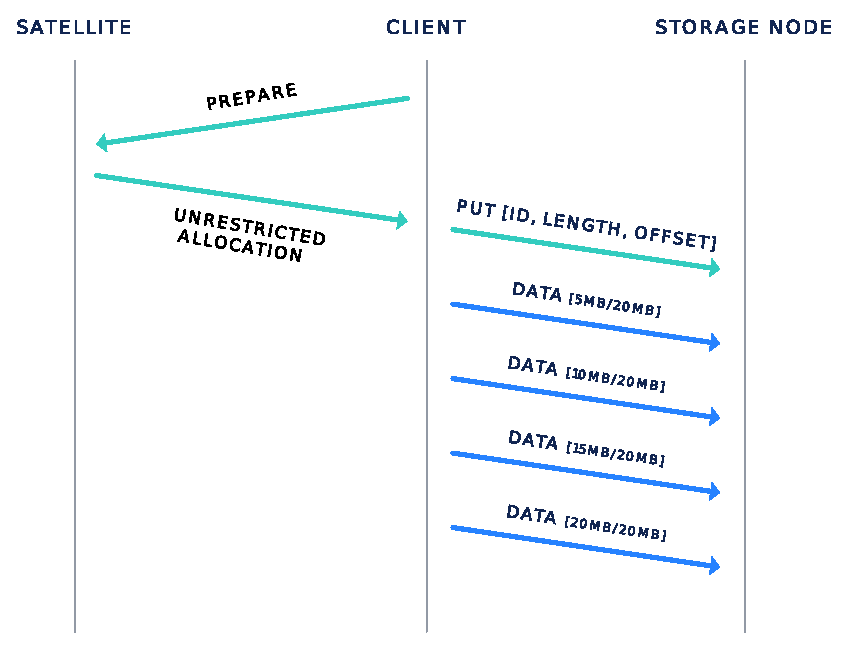
\includegraphics[height=.4\textheight]{images/put.eps}
\caption{Diagram of a put operation}
\label{fig:bap-put}
\end{figure}

\begin{figure}[!htbp]
\centering
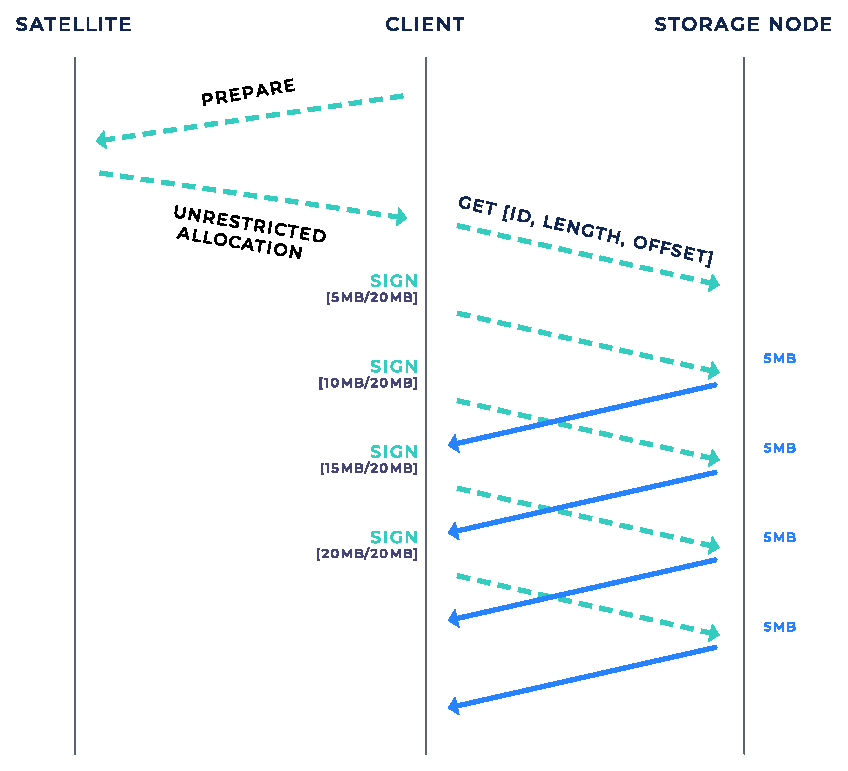
\includegraphics[height=.4\textheight]{images/get.eps}
\caption{Diagram of a get operation}
\label{fig:bap-get}
\end{figure}

A core component of our system requires knowing how much bandwidth is used
between two peers.

In our previous version \cite{storj-v2, sip9}, we used
{\em exchange reports} to gather information about what transpired between
two peers. At the end of an operation, both peers would send reports to a
central collection service for settlement. When both peers mutually agreed,
it was straightforward to determine how much bandwidth had been used.
When they disagreed, however, we resorted to data analysis and regression to
determine which peer had a greater propensity for dishonesty in an effort to
``catch cheaters.''
With our new version, we want to make cheating impossible from the protocol
level.

To solve this problem, we turn to Neuman's {\em Proxy-based authorization
and accounting for distributed systems} \cite{proxy-accounting}. This accounting
protocol more correctly measures resource usage in a delegated and decentralized
way.

In Neuman's accounting protocol, if an account holder has enough funds to
cover the operation, an account server will create a signed,
digital check and transfer it to the account holder.
The protocol refers to this check as a {\em proxy}, but we refer
to it as a {\em bandwidth allocation}. This check contains information
identifying the account server, the payer, the payee, the maximum amount of
resources available to be used in the operation, a check number to prevent
any double spending problems \cite{schneier}, and an expiration date.

In our case, the account server is the
Satellite, the payer is the Uplink, the payee is the storage node, and the
resource in question is bandwidth. The Satellite will only create a bandwidth
allocation if the Uplink is authorized for the request.
At the beginning of a storage operation, the Uplink can transfer the bandwidth
allocation to a storage node. The storage node can validate the Satellite's
signature and perform the requested operation up to the allowed bandwidth
limit, storing and later sending the bandwidth allocation to the Satellite for
payment. Because each Uplink already has a key pair as part of its identity
(section \ref{sec:node-id}), we use the existing key pair instead of
creating a new key pair for every bandwidth allocation.

We're further inspired by Filecoin's off-chain retrieval market,
wherein only small amounts of data are transferred at a time \cite{filecoin}.
Instead of allowing the storage node to cheat and save the bandwidth allocation
without performing the requested operation,
we break each operation into smaller requests such that if either the storage
node or Uplink stop participating in the protocol prematurely, neither peer
class is exposed to too much loss. This is similar to an optimistic, gradual
release, fair exchange protocol \cite{schneier}.

To support this with Neuman's accounting protocol and little Satellite overhead,
we use {\em restricted bandwidth allocations}
(referred to as {\em restricted proxies} in \cite{proxy-accounting}).
Neuman's restricted proxies work much like Macaroons
\cite{macaroons} in which further caveats can be added in a way that can't be
removed, limiting the capabilities of the proxy. Unlike Macaroons, proxies
can use public/private key cryptography, which means that anyone can validate
the proxy, instead of just the original issuer.

Restricted bandwidth allocations, in our case, are restricted by the Uplink to
limit the bandwidth allocation's value to only what has transferred so far.
In this way, the storage node will only keep the largest bandwidth allocation
it has received up to that point, and the Uplink will only send bandwidth allocations
that are slightly larger than what it has received.
The storage node has no incentive to keep more than the largest allocation, as
they all share the same ``check number,'' which can only be cashed once.

In the case of a {\em Get} operation, assume the Satellite-signed bandwidth
allocation allows up to $x$ bytes total. The Uplink
will start by sending a restricted allocation for some small amount ($y$ bytes),
perhaps only a few kilobytes,
so the storage node can verify the Uplink's authorization.
If the allocation is signed correctly, the storage node will
transfer up to the amount listed in the restricted allocation ($y$ bytes) before
awaiting another allocation. The Uplink will then send another allocation where
$y$ is larger, continuing to send allocations for data until $y$ has grown to
the full $x$ value.
For each transaction, the storage node only sends previously-unsent data,
so that the storage node only sends $x$ bytes total.
As seen in figure \ref{fig:bap-get},
we pipeline these requests to avoid pipeline stall performance penalties.

If the request is terminated at any time,
either planned or unexpectedly,
the storage node will keep the largest restricted bandwidth allocation it has
received.
This largest restricted bandwidth allocation is the signed confirmation
by the Uplink that the Uplink agreed to bandwidth usage of up to $y$
bytes, along with the Satellite's confirmation of the Uplink's bandwidth
allowance.
The storage node will periodically send the largest restricted bandwidth
allocations it has received to appropriate Satellites, at which point
Satellites will pay the storage node for that bandwidth.

If the Uplink can't afford the bandwidth usage, the Satellite will not sign an
bandwidth allocation, protecting the Satellite's reputation.
Likewise, if the Uplink tries to use more bandwidth than allocated,
the storage node will decline the request.
The storage node can only get paid for the maximum amount a client has agreed to,
as it otherwise has no valid bandwidth allocations to return for payment.

As before, we don't measure all peer-to-peer traffic;
this bandwidth traffic measurement system only tracks
bandwidth used during storage operations, storage and retrievals of pieces,
and does not apply to node discovery traffic (Kademlia DHT) or other generic
maintenance overhead.

\section{Satellite reputation}\label{sec:concrete-satellite-reputation}

Whenever a Satellite on the Storj network has a less than stellar payment,
demand generation, or performance history,
there is a strong incentive for the storage nodes to avoid accepting its data.

When a new Satellite joins the network, the participating storage nodes will
commence their own vetting process.
This process limits their exposure to the new and unknown
Satellite, while building trust over time to highlight which of the
Satellites have the best payment record.
Storage nodes will be able to configure the maximum amount of data they will
store for an untrusted Satellite, and will build historical data on whether
that Satellite will be trusted further in the future.
Storage node operators will also retain manual control on what Satellites they
will trust, or won't trust, if desired.

Storage node operators can elect to automatically trust a Storj Labs
provided collection of recommended Satellites that adhere to a strict set of
quality controls and payment service level agreements (SLAs).
To protect storage node operators, if a Satellite operator wants to be
included in the ``Tardigrade'' approved list,
the Satellite operator may be required to
adhere to a set of operating, payment, and pricing parameters and to sign a
business arrangement with Storj Labs.
See section \ref{sec:qc} for more details.

\section{Garbage collection}\label{sec:garbage-collection}

When clients move or delete data, clients, on behalf of Satellites, will notify
storage nodes
that they are no longer required to store that data.
When delete messages are issued via the client, the metadata system (and thus a
Satellite, with Satellite reputation on the line) will require proof that
deletes were issued to a configurable minimum number of storage nodes.
This means that every time
data is deleted, storage nodes that are online and reachable will receive
notifications right away.

Storage nodes will sometimes be temporarily unavailable and will miss delete
messages. In these cases, unneeded data is considered
{\em garbage}. Satellites only pay for data that they expect to be stored. Storage
nodes with lots of garbage will earn less than they will
otherwise unless a garbage collection system is employed. For this reason, we
introduce garbage collection to free up space on storage nodes.

A garbage collection algorithm is a method for freeing no-longer used resources.
A {\em precise} garbage collector collects all garbage exactly and
leaves no additional garbage. A {\em conservative} garbage collector, on the
other hand, may
leave some small proportion of garbage around given some other trade-offs,
often with the aim of improving performance.
As long as a conservative garbage collector is used in our system, the payment for
storage owed to a storage node will be high enough to amortize the cost of
storing the garbage.

For the nodes that miss initial delete messages, we propose a conservative
garbage collection strategy. Periodically, storage nodes will request
a data structure to detect differences. In the simplest form, it can be a hash
of stored keys, which allows efficient detection of out-of-sync state. After
detecting out-of-sync state, collection can use another structure, such as a
Bloom filter \cite{bloom-filter}, to find out what data has not been
deleted.
By returning a data
structure tailored to each node on a periodic schedule, a Satellite can give a
storage node the ability to clean up garbage data to a configurable tolerance.
Satellites will reject overly frequent requests for these data structures.

\section{Uplink}

Uplink is the term which we use to identify any software or service that invokes {\em libuplink} in order to interact with Satellites and storage nodes. It comes
in a few forms:

\begin{description}
\item[libuplink] - {\em libuplink} is a library that
  provides access to storing and retrieving data in the Storj network.

\item[Gateways] - Gateways act as compatibility layers between a service or
  application and the Storj network.
  They run as a service co-located with wherever data is generated, and will
  communicate directly with storage nodes so as to avoid central bandwidth
  costs.
  The Gateway is a simple service layer on top of {\em libuplink}.

  Our first gateway is an Amazon S3 gateway. It provides an S3-compatible,
  drop-in interface for users and applications that need to store data but
  don't want to bother with the complexities of distributed storage directly.

\item[Uplink CLI] - The Uplink CLI is a command line application which
  invokes {\em libuplink} allowing its user to upload and download files,
  create and remove buckets, manage file permissions, and other related tasks.
  It aims to provide an experience familiar to what you might expect when
  using Linux/UNIX tools such as {\em scp} or {\em rsync}.
\end{description}

Like storage nodes and Satellites,
the Uplink software in all three forms has been developed and released as
open source software.

\section{Quality control and branding}\label{sec:qc}

The Storj Network has two major product focuses that serve two distinct
target markets. These focal points are:

\begin{enumerate}
\item creating storage {\em supply} for the network via recruiting storage node
  operators and
\item creating {\em demand} for cloud storage with paying users.
\end{enumerate}

Storj will differentiate these focuses and the experience design
for each market segment by separating the supply side of our business from the
demand side through two brands, {\em Storj} and {\em Tardigrade}.

The supply side of the market will be served by the Storj brand.
We will retain \url{storj.io} as the place for contributing extra storage and
bandwidth to the Storj Network. This includes storage node setup, documentation,
frequently asked questions (FAQs), and tutorials. Users of both brands will also be able to
access our source code and community through \url{storj.io}.

The demand side of our business will be served by the Tardigrade brand and
will be directed through \url{tardigrade.io}.
This experience will be focused toward our partners and customers who purchased
decentralized storage and bandwidth from the network with the expectation of
high durability, resilience, and reliability, backed by an industry-leading
service level agreement (SLA). This includes any offers, free trials, Satellite
selection, documentation, FAQs, tutorials, and so forth.

The ``Tardigrade'' brand will additionally serve as a Satellite quality
credentialing system. Anyone can set up a Satellite via
\url{storj.io}, but to have a Satellite listed as an official Tardigrade
Satellite, be considered ``Tardigrade quality,'' and benefit directly from
Storj Labs' demand generation activities, an operator must pass
certain compliance and quality requirements.
These quality controls will continuously audit and rank Satellites on their
behavior, durability, compliance, and performance.
In addition, the Satellite operator will have to adhere to particular business
policies around pricing, storage node recruitment, SLAs, storage node payments,
and so forth.

Satellite operators in the Tardigrade network will have a business
relationship with Storj Labs that defines, among other things, franchise fees
and revenue sharing between the entities. Storj Labs will also assume
responsibilities including demand generation, brand enforcement, Satellite
operator support, end user support, United States Form 1099 tax filing
compliance,\footnote{US Form 1099 is required by law for any payments to an
individual in a given year exceeding a total of \$600.}
insurance, and maintenance of overall network quality.

These compliance and quality controls will be implemented to ensure that
storage nodes are fairly paid and Satellites are able to continuously meet all
SLAs of the Tardigrade products.

\chapter{Walkthroughs}\label{chap:walkthroughs}

The following is a collection of common use case examples of different types of
transactions of data through the system.

\section{Upload}

When a user wants to upload a file, the user first begins transferring data to
an instance of the Uplink.

\begin{itemize}
\item The Uplink chooses an encryption key and starting nonce for
  the first segment and begins encrypting incoming data with authenticated
  encryption as it flows to the network.
\item The Uplink buffers data until it knows whether the incoming segment is
short enough to be an inline segment or a remote segment. Inline segments are
small enough to be stored on the Satellite itself.
\end{itemize}

The rest of this
walkthrough will assume a remote segment because remote segments involve the
full technology stack.
\begin{itemize}
    \item The Uplink sends a request to the Satellite to prepare for the storage
of this first segment. The request object contains API credentials, such as
macaroons, and identity certificates.
\end{itemize}

Upon receiving the request, the Satellite will:
\begin{itemize}
\item Confirm that the Uplink has appropriate authorization and funds for
  the request. The Uplink must have an account with this specific Satellite
  already.
\item Make a selection of nodes with adequate resources that conform to the
  bucket's configured durability, performance, geographic, and reputation
  requirements.
\item Return a list of nodes, along with their contact information and
  unrestricted bandwidth allocation messages, and a chosen root piece ID.
\end{itemize}

Next, the Uplink will take this information and begin parallel connections to
  all of the chosen storage nodes while measuring bandwidth.

\begin{itemize}
\item The Uplink will begin breaking the segment into stripes and then
  erasure encode each stripe.
\item The generated erasure shares will be concatenated into {\em pieces} as they
  transfer to each storage node in parallel.
\item The erasure encoding will be configured to over-encode to more pieces
  than needed. This will eliminate the long tail effect and lead to a
  significant improvement of visible performance by allowing the Uplink to
  cancel the slowest uploads.
\item The data will continue to transfer until the maximum segment size is hit
  or the stream ends, whichever is sooner.
\item All of the hashes of every piece will be written to the end of each
  piece stream.
\end{itemize}

After that, the storage node will store: the largest restricted bandwidth allocation;
the TTL of the segment, if one exists; and the data itself. The data will
be identified by the storage node-specific piece ID and the delegating Satellite
ID.

If the upload is aborted for any reason, the storage node will keep the
largest restricted bandwidth allocation it received from the client Uplink on
behalf of the Satellite, but will throw away all other relevant request data.

Assuming success:

\begin{itemize}
\item The Uplink encrypts the random encryption key it chose for this file
  utilizing a deterministic hierarchical key.
\item The Uplink will upload a {\em pointer} object back to the Satellite, which
  contains the following information:
  \begin{itemize}
  \item which storage nodes were ultimately successful
  \item what encrypted path was chosen for this segment
  \item which erasure code algorithm was used
  \item the chosen piece ID
  \item the encrypted encryption key and other metadata
  \item a signature
  \end{itemize}
\end{itemize}

Finally, the Uplink will then proceed with the next segment, continuing to
process segments until the entire stream has completed. Each segment gets
a new encryption key, but the segment's starting nonce monotonically increases
from the previous segment.

\begin{itemize}
\item The last segment stored in the stream will contain additional metadata:
  \begin{itemize}
  \item how many segments the stream contained
  \item how large the segments are, in bytes
  \item the starting nonce of the first segment
  \item file extended attributes and other metadata
  \end{itemize}
\end{itemize}

Periodically, the storage nodes will later send the largest restricted
bandwidth allocation they received as part of the upload to the appropriate
Satellite for payment.

If an upload happens via the Amazon S3 multipart upload interface, each
{\em part} is uploaded as a segment individually.

\section{Download}

When a user wants to download a file, first the user sends a request for
data to the Uplink.
  The Uplink then tries to reduce the number of round trips to the Satellite
  by speculatively requesting the pointers for the first few segments in
  addition to the pointer for the last segment. The Uplink needs the last
  segment to learn the size of the object, the size and number of segments,
  and how to decrypt the data.

For every segment pointer requested, the Satellite will:
  \begin{itemize}
  \item Validate that the Uplink has access to download the segment pointer
    and has enough funds to pay for the download.
  \item Generate an unrestricted bandwidth allocation for each piece that
    makes up the segment.
  \item Look up the contact information for the storage nodes listed in the
  pointer.
  \item Return the requested segment pointer, the bandwidth allocations, and
    node contact info for each piece.
  \end{itemize}

The Uplink will determine whether more segments are necessary for the
  data request it received, and will request the remaining segment pointers if needed.

\begin{itemize}
\item Once all necessary segment pointers have been returned, if the requested
  segments are not inline, the Uplink will initiate parallel requests
  while measuring bandwidth (section \ref{baer}) to all appropriate storage
  nodes for the appropriate erasure share ranges inside of each stored piece.
\item Because not all erasure shares are necessary for recovery, long tails
  will be eliminated and a significant and visible performance improvement will
  be gained by allowing the Uplink to cancel the slowest downloads.
\item The Uplink will combine the retrieved erasure shares into stripes and
  decrypt the data.
\end{itemize}

If the download is aborted for any reason, each storage node will keep the
  largest restricted bandwidth allocation it received, but it will throw away all
  other relevant request data.
Either way, the storage nodes will later send the largest restricted
  bandwidth allocation they received as part of the download to the appropriate
  Satellite for later payment.

\section{Delete}

When a user wants to delete a file, the delete operation is first recieved
by the Uplink. The Uplink then requests all of the segment pointers for the file.

For every segment pointer, the Satellite will:
  \begin{itemize}
  \item Validate that the Uplink has access to delete the segment pointer.
  \item Generate a signed agreement for the deletion of the segment, so the
    storage node knows the Satellite is expecting the delete to proceed.
  \item Look up the contact information for the storage nodes listed in the
  pointer.
  \item Return the segments, the agreements, and contact information.
  \end{itemize}

For all of the remote segments, the Uplink will
  initiate parallel requests to all appropriate storage nodes to signal that the
  pieces are being removed.

\begin{itemize}
\item The storage nodes will return a signed message indicating the storage node
received the
delete operation and will delete both the file and its bookkeeping information,
or that it was already removed.
\item The Uplink will upload all of the signed messages that it received from
  working storage nodes back to the Satellite. The Satellite will require an
  adjustable percent of the total storage nodes to successfully sign messages
  to ensure that the Uplink did its part in notifying the storage nodes that the
  object was deleted.
\item The Satellite will remove the segment pointers and stop charging the
  customer and stop paying the storage nodes for them.
\item The Uplink will return a success status.
\end{itemize}

Periodically, storage nodes will ask the Satellite for generated garbage
  collection messages that will update storage nodes who were offline during the
  main deletion event.
  Satellites will reject requests for garbage collection messages that
  happen too frequently. See section \ref{sec:garbage-collection} for more
  details.

\section{Move}

When a user wants to move a file,
first, the Uplink receives a request for moving a file to a new path.
Then, the Uplink requests all of the segment pointers of that file.

For every segment pointer, the Satellite:
  \begin{itemize}
  \item Validates that the Uplink has access to download it.
  \item Returns the requested segment metadata.
  \end{itemize}

For every segment pointer, the Uplink:
  \begin{itemize}
  \item Decrypts the metadata with an encryption key derived from the path.
  \item Calculates the path at the new destination.
  \item Re-encrypts the metadata with a new encryption key derived from the
    new path.
  \end{itemize}

 The Uplink requests that the Satellite add
  all modified segment pointers and remove all old segment pointers in an
  atomic compare-and-swap operation.

The Satellite will validate that:
\begin{itemize}
\item The Uplink has appropriate authorization to remove the old path and create
  the new path.
\item The content of the old path hasn't changed since the overall operation
  started.
\end{itemize}

If the validation is successful, the Satellite will perform the operation.
 No storage node will receive any request related to the file move.

Because of the complexity around atomic pointer batch modifications, efficient
move operations may not be implemented right away.

\section{Copy}

When a user wants to copy a file, first, the Uplink receives a request for
copying a file to a new path.
Then the Uplink requests all of the segment pointers of the file.

For every segment pointer, the Satellite:
  \begin{itemize}
  \item Validates that the Uplink has access to download it.
  \item Looks up the contact information for the storage nodes listed in the
    pointer.
  \item Returns the requested segment metadata, a new root piece ID, and
    contact information.
  \end{itemize}

For every segment pointer, the Uplink:
  \begin{itemize}
  \item Decrypts the metadata with an encryption key derived from the path.
  \item Changes the path to the new destination.
  \item Invokes a copy operation on each of the storage nodes from the pointer
    to duplicate the piece with a new piece ID.
  \item Waits for the storage nodes to respond that they have duplicated the
    data, and removes nodes that were unsuccessful.
  \item Re-encrypts the metadata with the new piece ID and a new encryption key
    derived from the new path.
  \end{itemize}

Finally, the Uplink uploads all modified segment pointers to the Satellite.

Importantly, it is okay if the storage nodes de-duplicate storage, or only
store one actual copy of the data. All that matters is that the storage node
can identify the data by both the old and new piece ID. If one of the piece
IDs receives a delete operation, the other piece ID will continue working.
Only after both pieces are deleted will the node free the space.

\section{List}

When a user wants to list files:

\begin{itemize}
\item First, a request for listing a page of objects is received by the Uplink.
\item Then, the Uplink will translate the request on unencrypted paths to encrypted
  paths.
\item Next, the Uplink will request from the Satellite the appropriate page of
  encrypted paths.
\item After that, the Satellite will validate that the Uplink has appropriate access
  and then return the requested list page.
\item Finally, the Uplink will decrypt the return results and return them.
\end{itemize}

\section{Audit}

Each Satellite has a queue of segment stripes that will be audited across
  a set of storage nodes. The queue is filled via two mechanisms.
  \begin{itemize}
  \item In the first mechanism, the Satellite populates the queue periodically
    by selecting segments randomly, and then stripes within those segments also
    at random. Because segments have a maximum size, this sufficiently
    approximates our goal of choosing a byte to audit uniformly at random.
  \item In the second mechanism, the Satellite chooses a stripe to audit by
    identifying storage nodes that have had fewer recent audits than other
    storage nodes. The Satellite will select a stripe at random from the data
    contained by that storage node.
  \end{itemize}

Satellites will then work to process the queue and report errors.
\begin{itemize}
\item For each stripe request, the Satellite will perform the entire download
  operation for that small stripe range, filtering out nodes that are in
  containment mode. Unlike standard downloads, the stripe
  request does not need to be performant. The Satellite will attempt to
  download all of the erasure shares for the stripe and will wait for slow
  storage nodes.
\item After receiving as many shares as possible within a generous timeout,
  the erasure shares will be analyzed to discover which, if any, are wrong.
  Satellites will take note of storage nodes that return invalid data, and if a
  storage node returns too much invalid data, the Satellite will disqualify
  the storage node from future exchanges. In the case of a disqualification,
  the Satellite will not pay the storage node going forward, and it will not
  select the storage node for new data.
\item For storage nodes that did not respond, a cryptographic checksum of the
  expected audit result will be created and stored, placing the unresponsive
  nodes in containment. While in containment, a node will continue to be
  given only the audit it was unresponsive for until it passes or is
  disqualified.
\end{itemize}

\section{Data repair}

The repair process has two parts. The first part detects unhealthy files, and
the second part repairs them. Detection is straightforward.

\begin{itemize}
\item Each Satellite will periodically ping every storage node it knows
about, either as part of the audit process or via standard node discovery ping operations.
\item The Satellite will keep track of nodes that fail to respond and mark
  them as down.
\item When a node is marked down or is marked bad via the audit process, the
  pointers that point to that storage node will be considered for repair.
  Pointers
  keep track of their minimum allowable redundancy. If a pointer is not stored
  on enough good, online storage nodes, it will be added to the repair queue.
\end{itemize}

A worker process will take segment pointers off the repair queue.
When a segment pointer is taken off the repair queue:

\begin{itemize}
\item The worker will download enough pieces to reconstruct the entire segment,
  along with the piece hashes stored with those pieces
  (see section \ref{sec:concrete-piece-hashes}).
  Unlike audits, only enough pieces for accurate repair are needed.
  Unlike streaming downloads, the repair system can wait for the entire segment
  before starting.
\item The piece hashes are validated against the signature in the pointer, and
  then the downloaded pieces are validated against the validated piece hashes.
  Incorrect pieces are thrown away and count against the source as failed audits.
\item Once enough correct pieces are recovered, the missing pieces are
  regenerated.
\item The Satellite selects some new nodes and uploads the new pieces to
  those new nodes via the normal upload process.
\item The Satellite updates the pointer's metadata.
\end{itemize}

\section{Payment}

The payment process works as follows:

\begin{itemize}
\item First, the Satellite will choose a roll-up period. This is a period of
  time---defaulting to a day---that payment for data at rest is calculated.
\item During each roll-up period, a Satellite will consider all of the files it
  believes are currently stored on each storage node. Satellites will keep track
of payments owed to each storage node for each rollup period, based on
the data kept on each storage node.
\item Finally, storage nodes will periodically send in bandwidth allocation reports.
\end{itemize}

When a
  Satellite receives a bandwidth allocation report, it calculates the owed
  funds along with the outstanding data at rest calculations. It then sends the
  funds to the storage node's requested wallet address.

\chapter{Future work}\label{chap:future-work}

Storj is a work in progress, and many features are planned for future
versions. In this chapter we discuss a few especially interesting areas in
which we want to consider improvements to our concrete implementation.

\section{Hot files and content delivery}\label{sec:future-hot-files}

Occasionally, users of our system may end up delivering files that are more
popular than anticipated. While storage node operators might welcome the
opportunity to be paid for more bandwidth usage for the data they already have,
demand for these popular files might outstrip available bandwidth capacity,
and a form of dynamic scaling is needed.

Fortunately, Satellites already authorize all accesses to pieces, and
can therefore meter and rate limit access to popular
files. If a file's demand starts to grow more than current resources can serve,
the Satellite has an opportunity to temporarily pause accesses if necessary,
increase the redundancy of the file over more storage nodes, and then continue
allowing access.

Reed-Solomon erasure coding has a very useful property. Assume a $(k, n)$
encoding, where any $k$ pieces are needed of $n$ total. For any non-negative
integer number $x$, the first $n$ pieces of a $(k, n+x)$ encoding are the exact
same pieces as a $(k, n)$ encoding. This means that redundancy can easily be
scaled with little overhead.

As a practical example, suppose a file was encoded via a $(k=20, n=40)$ scheme,
and a Satellite discovers that it needs to double bandwidth resources to meet demand.
The Satellite can download any 20 pieces of the 40, generate just the last 40
pieces of a new $(k=20, n=80)$ scheme, store the new pieces on 40 new nodes,
and---without changing any data on the original 40 nodes---store the file
as a $(k=20, n=80)$ scheme, where any 20 out of 80 pieces are needed.
This allows all requests to adequately load balance across the 80 pieces.
If demand outstrips supply again, only 20 pieces are needed to generate even
more redundancy. In this manner, a Satellite could temporarily increase
redundancy to $(20, 1000)$, where requests are load balanced across 1,000 nodes,
such that every piece of all 1,000 are unique, and any 20 of those pieces are
all that is required to regenerate the original file.

The Satellite will need to pay storage nodes for the increased redundancy, so
content delivery in this manner has increased at-rest costs during high
demand, in addition to bandwidth costs. On the other hand, content delivery is often
desired to be highly geographically redundant, which this scheme provides
naturally.

\section{Improving user experience around metadata}\label{sec:distributed-metadata}

In our initial concrete implementation, we place significant burdens on the
Satellite operator to maintain a good service level with high availability,
high durability, regular payments, and regular backups. We expect a large
degree of variation in quality of Satellites, which led us to our quality
control program (see section \ref{sec:qc}).

Over time, clients of Satellites will want to reduce their dependence on Satellite
operators and enjoy more efficient data portability between Satellites besides
downloading and uploading their data manually. We plan to spend significant time
on improving this user experience in a number of ways.

In the short term, we plan to build a metadata import/export system, so users
can make backups of their metadata on their own and transfer their metadata
between Satellites.

In the medium term, we plan to reduce the size of these exports considerably
and make as much of this backup process as automatic and seamless as possible.
We expect to build a system to periodically back up the major portion of the metadata
directly to the network.

In the long term, we plan to architect the Satellite out of the platform.
We hope to eliminate Satellite control of the metadata
entirely via a viable Byzantine fault tolerant consensus algorithm, should
one arise.
The biggest challenge to this is finding the right balance between coordination
avoidance and Byzantine fault tolerant consensus, where storage nodes can
interact with one another, share encoded pieces of files, and still operate
within the performance levels users will expect from a platform that is
competing with traditional cloud storage providers.
Our team will continue to research viable means to achieve this end.

See section \ref{sec:coordination-avoidance} and
appendix \ref{chap:dist-consensus} for discussions on why we aren't tackling
the Byzantine fault tolerant consensus problem right away.

\chapter{Selected calculations}\label{chap:selected-calcs}

\section{Object repair costs}

A fundamental challenge in our system is how to not only choose the system
parameters that keep the expansion factor and repair bandwidth to a minimum but
also provide an acceptable level of durability.

Fortunately, we are not alone in wondering about this, and there is a good
amount of prior research on the problem.
``Peer-to-Peer Storage Systems: a Practical Guideline to be Lazy'' \cite{p2p-lazy} is an excellent guide, and much of our work follows from their conclusions.
The end result is a mathematical framework which determines network durability
and repair bandwidth given Reed-Solomon parameters, average node lifetime, and
reconstruction rate.

The following is a summary of results and explanation of their implications.

\begin{center}
\begin{tabular}{| c | c |}\hline
Variable & Description\\\hline
$MTTF$ & Mean time to failure \\
$\alpha$ & 1/$MTTF$\\
$MRT$ & Mean reconstruction time \\
$\gamma$ & 1/$MRT$\\
$D$&Total bytes on the network\\
$n$ & Total number of pieces per segment (RS encoding)\\
$k$ & Pieces needed to rebuild a segment (RS encoding)\\
$m$ & Repair threshold\\
$LR$ & Loss rate\\
1-$LR$ & Durability\\
$E_D$ & Expansion factor\\
$B_R$ & Ratio of data that is repair bandwidth\\
\hline
\end{tabular}
\end{center}

\begin{align*}
&&BW_R&=\frac{\alpha D(n-m+k)}{k\ln(n/m)}&\\
&&LR&=\frac{1}{(m+1)\ln(n/m)}\frac{m!}{(k-1)!}\left(\frac{\alpha}{\gamma}\right)^{m-k+2}&\\
&&E_D&=n/k&\\
&&B_R&=BW_R/D&\\
\end{align*}

The equations demonstrate that repair bandwidth is impacted by node churn
linearly, which is expected.
Lower mean time to node failure triggers more frequent rebuilds and,
therefore, more bandwidth usage.
Loss rate is much more sensitive to high node churn; it increases
exponentially with $\alpha$.
This necessitates very stable nodes, with lifetimes of several months, to
achieve acceptable network durability.
See section \ref{sec:RS} for a more in depth discussion of how node churn
affects erasure code parameters.

\subsection{Bandwidth limits usable space}\label{sec:bandwidth-space-limits}

Repair affects storage nodes' participation beyond their bandwidth usage; it
also constrains the amount of usable disk space.
Consider a storage node with 1 TB of available space, with a stated monthly
bandwidth limit of 500 GB.
If it's known (via the above framework) that a storage node can expect to
repair 50\% of its data in a given month, and assuming each stored object
is served at least once, then we can store no more than 333 GB on this node
since anything more than that causes more bandwidth than allowed.
In other words, paid bandwidth plus repair bandwidth must always be less than
or equal to the limit.

Higher repair rates equal lower effective storage size, but nodes serving paid
data more frequently are more sensitive to the effect.
In practice, the paid bandwidth rate will vary with the type of data being
stored on each node.
These ratios must be monitored closely to determine appropriate usable space
limits as the network evolves over time.

\pagebreak
\section{Audit false positive risk}\label{sec:audit-false-positive}

We rely on a Bayesian approach to determine the probability
that a storage node is maintaining stored pieces faithfully.
At a high level, we seek to answer the following question:
how do consecutive successful audits change our estimate of
the probability that a node will continue to return successful audits?

We model the audit process as being a binomial random variable
with an unknown probability of success $p\in[0,1]$, with each audit
being an independent Bernoulli trial.
It is well-known that the conjugate prior of the binomial distribution
is the beta distribution $\beta(a,b)$,
and that the posterior also follows the beta distribution.
As in \cite{tumor-occurrence},
we use the mean of the posterior distribution as our Bayes
estimator, which is given by $P=(a+x)/(a+b+n)$ where $a,b$ are the parameters of
the prior distribution, and $x$ is the number of successes observed in $n$ audits.
Under our assumption that each audit is successful,
we arrive at the Bayes estimate of the success probability $P=(a+n)/(a+b+n)$.

\begin{figure}[!htbp]
    \centering
    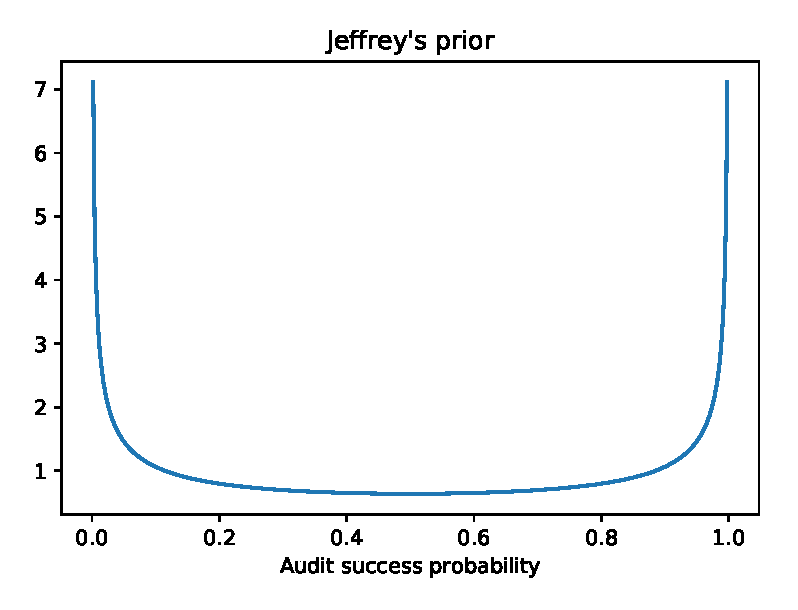
\includegraphics[height=.22\textheight]{audit-success/jeffrey_prior.eps}
    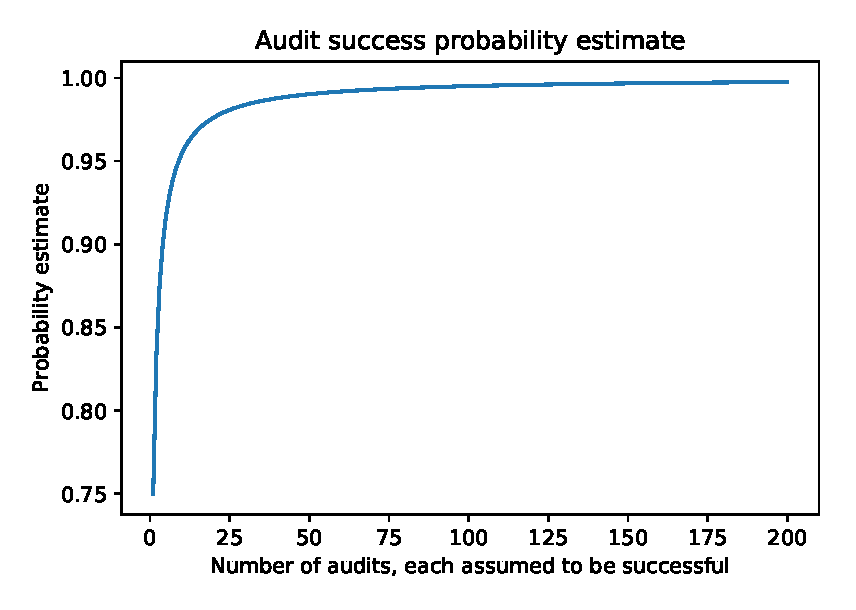
\includegraphics[height=.22\textheight]{audit-success/jeffrey_estimate.eps}
\caption{In Jeffrey's prior, we see the estimate for audit success probability is heavily weighted to be near 0 or near 1.}
\label{fig:jeff_prior}
\end{figure}

\begin{figure}[!htbp]
    \centering
    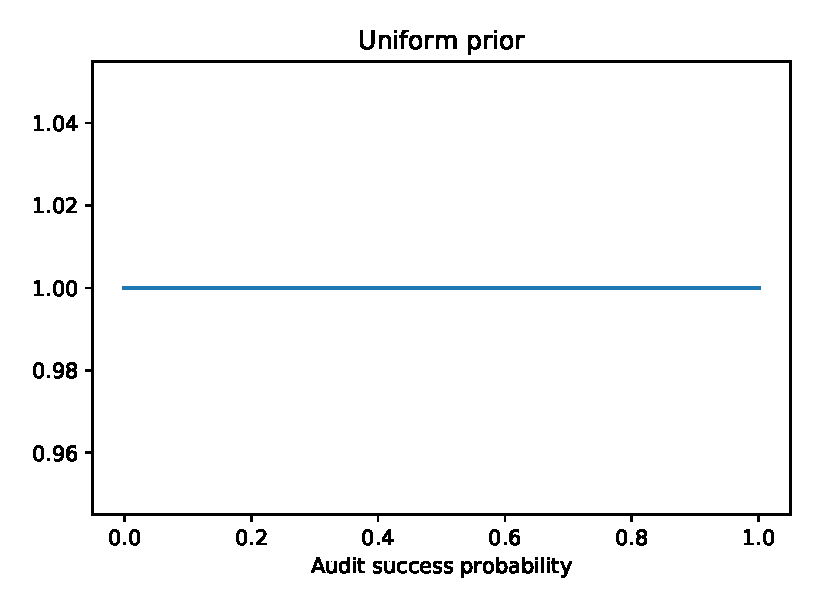
\includegraphics[height=.22\textheight]{audit-success/uniform_prior.eps}
    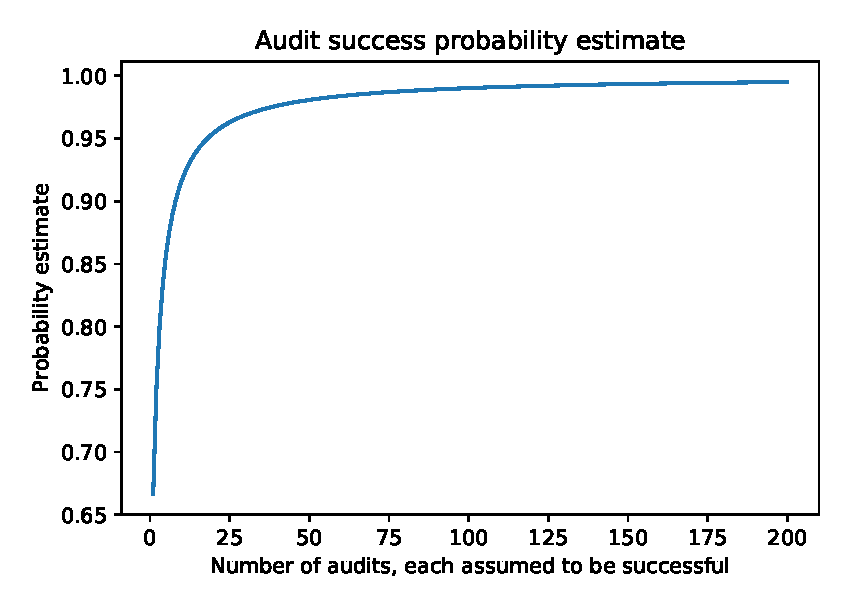
\includegraphics[height=.22\textheight]{audit-success/uniform_estimate.eps}
\caption{Using a Uniform prior, there is no assumption placed on the estimated
audit success probability, and all probabilities are assumed to be equally likely.}
\label{fig:unif_prior}
\end{figure}

We now choose a prior to derive a numerical estimate of the audit success probability
based on the number of audits performed.
There are many reasonable choices of Bayesian priors, but we restrict our attention to
two popular choices: the Uniform prior and Jeffrey's prior \cite{jeffrey}.
Using the Uniform prior $\beta(1,1)$ initializes the experiment
by assigning an equal probability to
all possible outcomes;
that is, the probability of success is drawn from the uniform
distribution on $(0,1)$.
Under Jeffrey's prior $\beta(0.5,0.5)$,
it is assumed that the probability of
success falls towards either extreme, so that a node will return a successful audit
either with probability near 0 or with probability near 1.

\begin{table}[!htbp]
\centering
\begin{tabulary}{\linewidth}{| C | C | C |}\hline
Number of audits & Audit success estimate given uniform prior & Audit success estimate given Jeffrey's prior\\\hline
0 & 0.5 & 0.5 \\
20 & 0.9545 & 0.9762 \\
40 & 0.9762 & 0.9878 \\
80 & 0.9878 & 0.9938 \\
200 & 0.99505 & 0.99751 \\
\hline
\end{tabulary}
\caption{Estimate of audit success probability by
number of audits, each assumed to be successful.
We find that the estimated probability of success begins at 0.5 when there is
no information known about the node (no audits have been performed),
with the estimate quickly jumping to above 99\% in as few as 80 audits using Jeffrey's prior.}
\label{table:audit-success-estimates}
\end{table}

In table \ref{table:audit-success-estimates},
we present results obtained from using both priors.
We remark that the well-established Bayesian approach
allows us to rapidly gain more confidence
in a node's ability to return a successful audit,
given that the success probability estimate tends closer to 1
with each consecutive audit success.
\FloatBarrier


\pagebreak
\section{Choosing erasure parameters}
\label{sec:RS}

\linespread{2.0}

In the context of storing an erasure-coded file on a decentralized network, we consider file piece loss from two different perspectives.

\section{Direct file piece loss}
With direct file piece loss, we assume that for a specific file, its erasure pieces are lost according to a certain rate. We point out that modeling this is straightforward: if file pieces are lost at a rate $0<p<1$ and we start with $n$ pieces, then file piece decay follows an exponential decay pattern of the form $n(1-p)^t$, with $t$ being the time elapsed according to the units used for the rate\footnote{So if we assume a proportion of $p=.1$ pieces are lost per month, $t$ is given in months.}.
To account for $a$ multiple checks per month, we may extend this to $n(1-p/a)^{at}$. If $m$ is the rebuild threshold which controls when a file is rebuilt, we may solve $n(1-p/a)^{at}=m$ for $t$ (taking the ceiling when necessary) to determine how long it will take for the $n$ pieces of a file to decay to less than $m$ pieces. This works out to the smallest $t$ for which
$t>\frac{\ln(m/n)}{a\ln(1-p/a)}$. Thus it becomes clear, given parameters $n,m,a$ and $p$, how long we expect a file to last between repairs.

\section{Indirect file piece loss}

When modeling indirect file piece loss, we suppose that a fixed rate of nodes
drop out of the network each month\footnote{Though the rate may be taken over
any desired time interval.}, whether or not they are holding pieces of the file
under consideration. To describe the probability that $d$ of the dropped nodes
were delegates for a specific file coded into $n$ pieces, we turn to the
Hypergeometric probability distribution. Suppose $c$ nodes are replaced per
month out of $C$ total nodes on the network. Then the probability that $d$
nodes were delegates for the file is given by
\begin{align}
    P(X=d)&=\frac{\binom{n}{d}\binom{C-n}{c-d}}{\binom{C}{c}}\label{hgeom}
\end{align}
which has mean $nc/C$. We then determine how long it will take for the number of pieces to fall below the desired threshold $m$ by iterating, holding the overall churn $c$ fixed but reducing the number of existing pieces by the distribution's mean in each iteration and counting the number of iterations required. For example, after one iteration, the number of existing pieces is reduced by $nc/C$, so instead of $n$ pieces on the network (as the parameter in \eqref{hgeom}), there are $n-nc/C$ pieces, changing both the parameter and the mean for \eqref{hgeom} in iteration 2.

We may extend this model by considering multiple checks per month (as in the direct file piece loss case), assuming that $c/a$ nodes are lost every $1/a$-th of a month instead of assuming that $c$ nodes are lost per month, where $a$ is the number of checks per month. This yields an initial Hypergeometric probability distribution with mean $nc/aC$.

In either of these two cases (single or multiple file integrity checks per month), we track the number of iterations until the number of available pieces fall below the repair threshold. This number may then be used to determine the expected number of rebuilds per month for any given file.


\subsection{Numerical simulations for indirect file piece loss}
\subsubsection{Introduction}
We produce decision tables showcasing worst-case mean file rebuild outcomes based on simulating file piece loss for files encoded with varying Reed-Solomon parameters. 
We assume an $(k,n)$ RS encoding scheme, where $n$ pieces are generated, with 
$k$ pieces needed for reconstruction, using three different values for $n$.
We assume that a file undergoes the process of repair when less than $r$ pieces remain on the network, using three different values of $m$ for each $n$.
For the initial table, we use a simplifying assumption that pieces on the network are lost at a constant rate per month\footnote{This constant rate may be viewed as the mean of the Poisson distribution modeling piece loss per month.}, which may be due to node churn, data corruption, or an alien megarace extracting a farmer's hard-drive to a higher dimension (amongst other possibilities).


To arrive at the value for mean rebuilds per month, we consider a single file that is encoded with $n$ pieces which are distributed uniformly randomly to nodes on the network. To simulate conditions leading to a rebuild, we uniformly randomly select a subset of nodes from the total population and designate them as failed. We do this multiple times per (simulated) month, scaling the piece loss rate linearly according to the number of file integrity checks (``checks") per month\footnote{
For example, if the monthly network piece loss rate is assumed to be 0.1 of the network size (or 10\%), and if 10 file integrity checks are performed per month, we assume that, on average, 1\% of pieces are lost between checks.}. 
Once enough nodes have failed to bring the number of file pieces under the repair threshold, the file is rebuilt, and we track the number of rebuilds over the course of 24 months.
We repeat this simulation for 1000 iterations, simulating 1000 2-year periods for a single file. We then take the number of rebuilds at the 99-th percentile (or higher) of the number of rebuilds occuring over these 1000 iterations. In other words, we choose the value for which the value of the observed CDF (describing the number of rebuilds over this 2 year period) is at least 0.99. This value is then divided by the number of months to arrive at the mean rebuilds/month value. An example of the approach is shown in Figure \ref{fig:sim_method}. We perform the experiment on a network of 10,000 nodes, observing that the network size will not directly impact the mean rebuilds/month value for a single file under our working assumption of a constant rate of loss per month\footnote{We represent piece loss as a proportion of nodes selected uniformly randomly from the total network. The proportion scales directly with network size, so the overall number of pieces lost stays the same for networks of different sizes.}.

\linespread{1}
\begin{figure}[h]
    \centering
    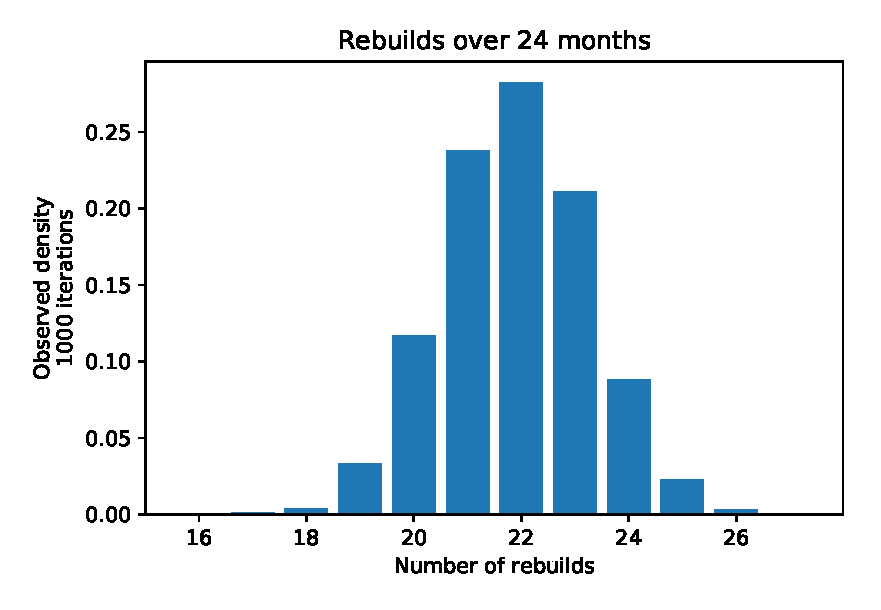
\includegraphics[scale=0.5]{RS-appendix-files/example_pmf.eps}
    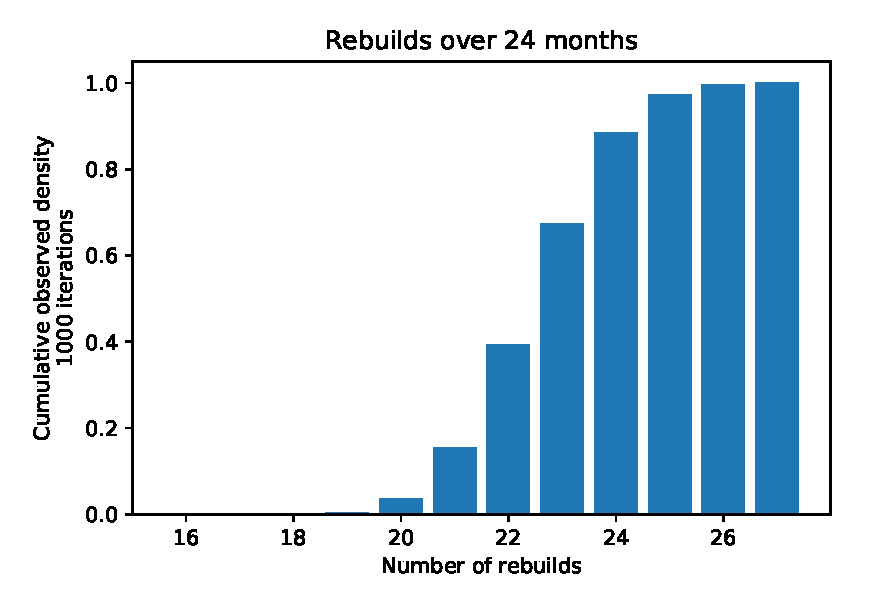
\includegraphics[scale=0.5]{RS-appendix-files/example_cdf.eps}
    \caption{Top: Density for the number of rebuilds over a 24 month period, repeated for 1000 iterations. Bottom: CDF of the number of rebuilds. In this case, the mean rebuilds/month value would be taken as $26/24\approx1.083$, with there being a 99.7\% chance that a file is rebuilt at most 26 times over the course of 24 months.}
    \label{fig:sim_method}
\end{figure}

\pagebreak
\linespread{1}
\pagebreak
\subsubsection{The decision tables}
In forming the decision tables, we consider as part of our calculations how
different choices of k, n, m, and mean time to failure affect durability and repair bandwidth. What we are looking for is the lowest repair bandwidth that also meets our
durability requirements.
\begin{table}[!htpb]\centering

\begin{tabular}{| c | c c c | c | c|}\hline
MTTF (months) &$k$& $n$ & $m$ &Repair Bandwidth Ratio&Durability (\# nines) \\\hline
1 &20& 40 & 35 & 9.36 & 0.9999 (8) \\
6 &20& 40 & 30 & 0.87 & 0.9999 (17) \\
12 &20& 40 & 25 & 0.31 & 0.9999 (13)\\\hline

1 &30& 60 & 35 & 3.40 &0.9999 (4)\\
6 &30& 70 & 40 & 0.60 &0.9999 (15)\\
12 &30& 80 & 45 & 0.31 &0.9999 (25) \\\hline

1 &40& 80 & 60 & 5.21 &0.9999 (4)\\
6 &40&120&50 & 0.52 &0.9999(14)\\
12 &40&120&45 & 0.24 &0.9999 (11)\\\hline

\end{tabular}
\caption{Decision tables showing the relationship between churn (MTTF),
  Reed-Solomon parameters ($k$, $n$, $m$), repair bandwidth ratio, and durability}
\label{rs:decision-tables}
\end{table}




\subsection{Making a decision}

We conclude by observing that these models may be tuned to target specific network scenarios and requirements. One network may require one set of Reed-Solomon parameters, while a different network may require another. In general, the closer $m/n$ is to 1, the more rebuilds per month should be expected under a fixed churn rate. While having a larger ratio for $m/n$ increases file durability for any given churn rate, it comes at the expense of more bandwidth used since repairs are triggered more often. To maintain a low mean rebuilds/month value while also maintaining a higher file durability, the aim should be to increase the value of $n$ as much as feasible given other network conditions (latency, download speed, etc.), which allows for a lower relative value of $r$ while still not jeopardizing file durability. 

Informally, it takes longer to lose more pieces under a given fixed network size and churn rate. Therefore, to maximize durability while minimizing repair bandwidth usage, $n$ should be as large as existing network conditions allow. This allows for a value of $m$ that is relatively closer to $k$, reducing the mean rebuilds/month value, which in turn lowers the amount of repair bandwidth used. 

For example, assume we have a network with a mean time to failure of six months.
Suppose we consider the same file encoded with two different RS parameters: 
one under a $(20,40)$ schema and the other as an $(30,80)$ schema. If we set $m$ so that $m=k+10$ for both cases, we observe from the above table
that the bandwidth repair ratio is is $0.87$ in the $(20,40)$ case and is $0.60$ in the $(40,80)$ case. Both encoding schemes have similar durability, as a repair in both cases is triggered when there are $k+10$ pieces left; even though, the mean rebuilds per month 
is empirically and theoretically lower for the $(40,80)$ case using $m=k+10$. 

\newpage \appendix
\addtocontents{toc}{\protect\setcounter{tocdepth}{0}}

\chapter{Distributed consensus}\label{chap:dist-consensus}

To discuss why we are not trying to solve byzantine distributed consensus,
it's worth a brief discussion of the history of distributed consensus.

\section{Non-byzantine distributed consensus}

Computerized data storage systems began by necessity with single computers
storing and retrieving data on their own. Unfortunately, in environments where
the system must continue operating at all times, a single computer failure can
grind an important process to a halt. As a result, researchers have often
sought ways to enable groups of computers to manage data
without any specific computer being required for operation. Spreading ownership
of data across multiple computers could increase uptime in the face of failures,
increase throughput by spreading work across more processors, and so forth.
This research field has been long and challenging; but, fortunately, it has led
to some really exciting technology.

The biggest issue with getting a group of computers to agree is that messages
can be lost. How this impacts decision making is succinctly described by the
``Two Generals' Problem'' \cite{two-generals},\footnote{
earlier described as a problem
between groups of gangsters \cite{two-gangsters}} in which two armies try to
communicate in the face of potentially lost messages. Both armies have already
agreed to attack a shared enemy, but have yet to decide on a time. Both armies
must attack at the same time or else failure is assured. Both armies can send
messengers, but the messengers are often captured by the enemy. Both armies must
know what time to attack and that the other army has also agreed to this time.

Ultimately, a generic solution to the two generals' problem with a finite number
of messages is impossible, so engineering approaches have had
to embrace uncertainty by necessity. Many distributed systems make trade-offs to
deal with this uncertainty. Some systems embrace {\em consistency}, which means
that the system will choose downtime over inconsistent answers. Other
systems embrace {\em availability}, which means that the system chooses
potentially inconsistent answers over downtime. The widely-cited CAP
theorem \cite{cap1, cap2} states that every system must choose only two of
consistency, availability, and partition tolerance.
Due to the inevitability of network
failures, partition tolerance is non-negotiable, so when a partition happens,
every system must choose to sacrifice either consistency or availability. Many
systems sacrifice both (sometimes by accident).

In the CAP theorem, consistency (specifically, linearizability) means that
every read receives the most recent write or an error, so an inconsistent
answer means the system returned something besides the most recent write
without obviously failing.
More generally, there
are a number of other {\em consistency models} that may be acceptable by making
various trade-offs. Linearizability, sequential consistency, causal consistency,
PRAM consistency, eventual consistency, read-after-write consistency, etc., are
all models for discussing how a history of events appears to various
participants in a distributed system.\footnote{If differing consistency models
are new to you, it may be worth reading about them in Kyle Kingbury's excellent
tutorial \cite{aphyr-consistency}. If you're wondering why computers can't just
use the current time to order events, keep in mind it is exceedingly difficult
to get computers to even agree on that \cite{no-now}.}

Amazon S3 generally provides {\em read-after-write consistency}, though in some
cases will provide {\em eventual consistency} instead \cite{s3-consistency}.
Many distributed databases provide eventual consistency by
default, such as Dynamo \cite{dynamo} and Cassandra \cite{cassandra}.

Linearizability in a distributed system is often much more desirable than more
weakly consistent models, as it is
useful as a building block for many higher level data structures and operations
(such as distributed locks and other coordination techniques). Initially, early
efforts to build linearizable distributed consensus centered around two-phase
commit, then three-phase commit, which both
suffered due to issues similar to the two generals' problem. In 1985,
the FLP-impossibility paper \cite{flp} proved that no algorithm
could reach linearizable consensus in bounded time. Then in 1988, Barbara Liskov
and Brian Oki published the Viewstamped Replication algorithm \cite{vr} which
was the first linearizable distributed consensus algorithm. Unaware of the VR
publication, Leslie Lamport set out to prove linearizable distributed consensus
was impossible \cite{paxos-note}, but instead in 1989 proved it was possible by
publishing his own Paxos algorithm \cite{paxos}, which for some reason became
significantly more popular. Ultimately both algorithms have a large amount in
common.

Despite Lamport's claims that Paxos is actually simple \cite{paxos-simple},
many papers have been published since then
challenging that assertion. Google's description of their attempts to implement
Paxos are described in Paxos Made Live \cite{paxos-live},
and Paxos Made Moderately
Complex \cite{paxos-complex} is an attempt to try and fill in all the details of
the protocol. The entire basis of the Raft algorithm is rooted in trying to
wrangle and simplify the complexity of Paxos \cite{raft}. Ultimately, after an
upsetting few decades, reliable implementations of Paxos, Raft, Viewstamped
Replication \cite{vrr}, Chain Replication \cite{chain-rep}, and Zab \cite{zab}
now exist, with ongoing work to improve the situation
further \cite{epaxos,paxos-flexible}. Arguably, part of Google's early success
was in spending the time to build their internal Paxos-as-a-service distributed
lock system, Chubby \cite{chubby}. Most of Google's famous early internal data
storage tools, such as Bigtable \cite{bigtable}, depend on Chubby for
correctness. Spanner \cite{spanner}---perhaps one of the most incredible
distributed databases in the world---is largely just two-phase commit on top of
multiple Paxos groups.

\section{Byzantine distributed consensus}

As mentioned in our design constraints, we expect most nodes to be {\em
rational} and some to be {\em byzantine}, but few-to-none to be {\em
altruistic}. Unfortunately, all of the previous algorithms we discussed assume a
collection of altruistic nodes.
Reliable distributed consensus algorithms have been game-changing for many
applications requiring fault-tolerant storage. However, success has been much
more mixed in the byzantine fault tolerant world.

There have been a number of attempts to solve the Byzantine fault tolerant
distributed consensus problem. The field exploded after the release of Bitcoin
\cite{bitcoin}, and is still in its early stages. Of note, we are particularly
interested in PBFT \cite{pbft} (Barbara Liskov again with the
first solution out of the gate), Q/U \cite{qu}, FaB \cite{fab} (but see
\cite{fab-revisited}), Bitcoin, Zyzzyva \cite{zyzzyva} (but also
see \cite{fab-revisited}), RBFT \cite{rbft}, Tangaroa \cite{tangaroa},
Tendermint \cite{tendermint}, Aliph \cite{aliph}, Hashgraph \cite{hashgraph},
HoneybadgerBFT\cite{honeybadger}, Algorand\cite{algorand}, Casper\cite{casper},
Tangle\cite{tangle}, Avalanche\cite{avalanche}, PARSEC\cite{parsec}, and
others\cite{mickens-bft}.

Each of these algorithms make
additional trade-offs, that non-Byzantine distributed consensus algorithms don't
require, to deal with the potential for uncooperative nodes. For example,
PBFT \cite{pbft} causes a significant amount of network overhead. In PBFT, every
client must attempt to talk to a majority of participants, which must all
individually reply to the client. Bitcoin
\cite{bitcoin} intentionally limits the transaction rate with changing
proof-of-work difficulty. Many other post-Bitcoin protocols require all
participants to keep a full copy of all change histories.

\section{Why we're avoiding Byzantine distributed consensus}

Ultimately, all of the existing solutions fall short of our goal of minimizing
coordination (see section \ref{sec:coordination-avoidance}). Flexible Paxos
\cite{paxos-flexible} does significantly better than normal Paxos in the
steady-state for avoiding coordination, but is completely unusable in a
byzantine environment. Distributed ledger or ``tangle-like'' approaches suffer
from an inability to prune history and retain significant global coordination
overhead.

We are excited and look forward to a fast, scalable byzantine fault tolerant
solution. The building blocks of one may already be listed in the previous
discussion. Until it is clear that one has arisen, we are reducing our risk
by avoiding the problem entirely.

\chapter{Attacks}

As with any distributed system, a variety of attack vectors exist. Many of these
are common to all distributed systems. Some are storage-specific and will apply
to any distributed storage system.

\section{Spartacus}

Spartacus attacks, or identity hijacking, are possible on unmodified Kademlia
\cite{kad}.
Any node may assume the identity of another node and receive some fraction of
messages intended for that node by simply copying its node ID.
This allows for targeted attacks against specific nodes and data.
Spartacus attack mitigation is addressed in S/Kademlia \cite{skad} by
implementing node IDs as public key hashes and requiring messages to be signed.
A Spartacus attacker in this system would be unable to generate the
corresponding private key, and thus unable to sign messages and participate in
the network.

\section{Sybil}

Sybil attacks involve the creation of large amounts of nodes in an attempt to
disrupt network operation by hijacking or dropping messages. Kademlia
\cite{kad} is already somewhat resistant to Sybil attacks, because
it relies on both message redundancy and a concrete distance metric.
A node's neighbors in the network are selected by
node ID from an evenly distributed pool, and most messages are sent to at least
$k$ neighbors. If a Sybil attacker controls 50\% of the network, it
successfully isolates only 12.5\% of honest nodes. While reliability and
performance will degrade, the network will still be functional unless a large
portion of the network consists of colluding Sybil nodes.

As an additional defense against sybil attacks, S/Kademlia \cite{skad}
extends Kademlia with a proof of work scheme, which we have adopted. See section
\ref{sec:node-id} for more details.

Our storage node reputation system involves a prolonged initial vetting
period nodes must complete before they are trusted with significant amounts
of data. This vetting system, discussed more in section
\ref{sec:concrete-reputation}, prevents a large influx of new nodes from taking
incoming data from existing reputable storage nodes without first proving
their longevity.

\section{Eclipse}

An eclipse attack attempts to isolate a node or set of node in the network
graph by ensuring that all outbound connections reach malicious nodes. Eclipse
attacks can be hard to identify, as malicious nodes can be made to function
normally in most cases, only eclipsing certain important messages or
information. Storj addresses eclipse attacks by using public key hashes as node
IDs, signatures based on those public keys, and multiple disjoint network
lookups as prescribed by S/Kademlia \cite{skad}.

The larger the network is, the harder it will
be to prevent a node from finding a portion of the network uncontrolled by
an attacker.
As long as a storage node or Satellite has been introduced to a portion of
the network that is not controlled by the attacker at any point, the public
key hashes and signatures ensure that man-in-the-middle attacks are impossible,
and multiple disjoint network lookups ensure that Kademlia routing is
prohibitively expensive to bias.

To avoid an eclipse attack, all that remains
is to make sure new nodes are appropriately introduced to at least one
well-behaved node on the network during the bootstrapping process.
To that end, Storj Labs will run some well-known, verified bootstrap nodes.

\section{Honest Geppetto}

In this attack,
the attacker operates a large number of ``puppet'' storage nodes on the network,
accumulating trust and contracts over time. Once a certain threshold is reached,
he pulls the strings on each puppet to execute a hostage attack with the data
involved, or simply drops each storage node from the network. The best defense
against this attack is to create a network of sufficient scale that this attack
is ineffective. In the meantime, this can be partially prevented by relatedness
analysis of storage nodes. Bayesian inference across downtime, latency, network
route, and other
attributes can be used to assess the likelihood that two storage nodes are
operated by the same organization. Satellites can and should attempt to
distribute pieces across as many unrelated storage nodes as possible.

\section{Hostage bytes}

The hostage byte attack is a storage-specific attack where malicious storage
nodes
refuse to transfer pieces, or portions of pieces, in order to extort additional
payments from clients. The Reed-Solomon encoding ought to be sufficient to
defeat attacks of this sort (as the client can simply download the necessary
number of pieces from other nodes) unless multiple malicious nodes collude to
gain control of many pieces of the same file. The same mitigations discussed
under the Honest Geppetto attack can apply here to help avoid this situation.

\section{Cheating storage nodes, Uplinks, or Satellites}

Measuring bandwidth with signatures minimizes the risk for Uplink and storage
nodes.
The Uplink can only interact with the storage node by sending a signed
restricted allocation.
The restriction limits the risk to a very low amount.
The storage node has to comply with the protocol as expected in order to get
more restricted allocations.
Storage nodes and Satellites will commence a vetting process that limits their
exposure.
Storage nodes are allowed to decline requests from untrusted Satellites.

\section{Faithless storage nodes and Satellites}

While storage nodes and Satellites are built to require authentication via
signatures before serving download requests, it is reasonable to imagine a
modification of the storage node or Satellite that will provide downloads to
any paying requestor.
Even in a network with a faithless Satellite, data privacy is not significantly
compromised.
Strong client-side encryption protects the contents of the file from
inspection.
Storj is not designed to protect against compromised clients.

\section{Defeated audit attacks}

A typical Merkle proof verification requires pre-generated challenges and
responses.
Without a periodic regeneration of these challenges, a storage node can begin
to pass most audits without storing all of the requested data.
Instead, we request a random stripe of erasure shares from all storage nodes.
We run the Berlekamp-Welch algorithm\cite{bw} across all the
erasure shares.
When enough storage nodes return correct information, any faulty or missing
responses can easily be identified.
New storage nodes will be placed into a vetting process until enough audits
have passed.

See section \ref{sec:concrete-reputation} for more.

\chapter{Primary user benefits}

We have designed the Storj network to provide users better security,
availability, performance, and economics---across a wide variety of use
cases---than either on premises storage solutions or traditional, centralized
cloud storage. While the bulk of the paper describes the design considerations
to overcome the challenges of a highly decentralized system, this appendix
describes why the end result should be a significant improvement over
traditional approaches.

\section{Security}

We have designed our system to be the equivalent of spreading encrypted sand
on an encrypted beach. All data is encrypted client side before reaching our
system. Data is sharded and distributed across a large number of independently
operated disk drives which are part of a much larger network of independently
operated storage nodes.

In a typical scenario (with a 20/40 Reed-Solomon
setup), each file is distributed across 40 different disk drives in a global
network of over 100,000 independently operated nodes. (The previous version of
the Storj network had over 150,000 independently operated nodes.) To compromise
an individual file, a would-be bad actor would have to locate and compromise
roughly 40 different drives, each operated by a different provider, in a
network of over 100,000 drives. Even if the actor were somehow able to
compromise those drives, to reconstruct the file, the would-be bad-actor would
then have to decrypt 256-bit AES encrypted data, with keys that are only held
by the end user. And, the would-be bad actor would have to repeat this process
with an entirely different set of potential drives for the next file they wish
to obtain.

By design, it is not possible for Storj, Satellite operators,
storage node operators, or would-be bad actors to mine or compromise end user
data. The level of decentralization creates powerful disincentives for
malicious actors, as there is no centralized trove of data to target.

\section{Availability}

While most centralized cloud providers employ various strategies to provide
protection against individual drive failures, they are not immune to
system-wide events. Storms, power outages, floods, earthquakes, operator error,
design flaws, network overload, or attacks can compromise entire data centers.

While the centralized providers may calculate and publish theoretically high
availability numbers, these calculations depend on drive failures being
uncorrelated. In fact, in any data center, the chances of an individual drive
failing is highly correlated with the chances of another drive failing.

In a decentralized system, by contrast, each node is operated by a different
individual, in a different location, with separate personnel, power, network
access, etc. Thus, the chance of an individual node failing is almost entirely
uncorrelated with the chances of other drives failing. As a result, the kinds
of availability we obtain are not subject to storms, power outages, or other
``black swan'' events. Even if the chance of an individual drive failing in the
Storj network is higher than in a centralized cloud, the chance of collective
failure (e.g. losing 20 out of 40 independent drives) is vanishingly small.
And, the chance of losing one file is not correlated with the chances of
losing a second file.

\section{Performance}

For read-intensive use cases, the Storj network can deliver superior
performance by taking advantage of parallelism. The storage nodes are located
close to ``the edge,'' reducing the latency experienced when recipients of
data are physically far from the data center that houses the data.
Read performance benefits from parallelism. The particular erasure coding
scheme that we use ensures that slow drives, slow networks, or networks and
drives experiencing temporarily high load do not limit throughput. We can
adjust the $k/n$ ratio so that we dramatically improve download and streaming
speeds, without imposing the kinds of high costs associated with CDN networks.

\section{Economics}

While the amount of data created has doubled every year, the price of cloud
storage has only declined about 10\% per year over the last three years.
There are a number of potential explanations, both on the supply and demand
side.

Public cloud storage operators must make large capital investments in
building out a network of data centers and must incur significant costs for
power, personnel, security, fire suppression, etc. Their pricing structure
must allow them to recoup those costs. Moreover, the structure of the
industry is such that it is inherently oligopolistic: there are only a
handful of public cloud companies, and they comprise the largest companies by
market cap on the planet (Microsoft, Google, Amazon, Alibaba).
As any price decreases by one provider are quickly matched by the other
providers, there has been little incentive for providers to drop prices to
gain market share.

In a decentralized network, by contrast, there is little
marginal cost to being a storage node operator. In our experience, the vast
majority of operators are using existing live equipment with significant spare
capacity. There is no additional cost to a storage node operator in terms of
capital or personnel. Running a drive at low capacity does not consume
significantly more power than running a drive at near full capacity. And, with
careful management relative to caps, most operators do not experience
increased bandwidth costs. Consequently, operating a node represents nearly
pure margin, and these supply cost savings can be passed on to end users.

We have designed market mechanisms on the demand side as well, to prevent any
Satellite operator from cornering the market. Even after providing a healthy
margin to farmers, demand partners, and Satellite operators, we believe we
hould be able to provide storage services profitably at a fraction of the cost
of equivalent centralized cloud services.

\newpage
\bibliographystyle{unsrt}
\begingroup
\raggedright
\bibliography{biblio}
\endgroup

\end{document}
